% LaTeX Template for Project Report, Version 2.0
% (Abstracted from a Major Project Report at CSED, NIT Calicut but can be
% modified easily to use for other reports also.)
%
% Released under Creative Commons Attribution license (CC-BY)
% Info: http://creativecommons.org/licenses/by/3.0/
%
% Created by: Kartik Singhal
% BTech CSE Batch of 2009-13
% NIT Calicut
% Contact Info: kartiksinghal@gmail.com
%
% It is advisable to learn the basics of LaTeX before using this template.
% A good resource to start with is http://en.wikibooks.org/wiki/LaTeX/
%
% All template fields are marked with a pair of angular brackets e.g. <title here>
% except for the ones defining citation names in ref.tex.
%
% Empty space after chapter/section/subsection titles can be used to insert text.
%
% Just compile this file using pdflatex after making all required changes.

\documentclass[12pt,a4paper]{report}
\usepackage{fullpage}
\usepackage{hyperref}
\usepackage{color}
\usepackage{placeins}
\usepackage[pdftex]{graphicx}
\usepackage{todonotes}
\usepackage{ourmacros}
\usepackage{listings}
\usepackage{amsfonts}
\usepackage{url}
\usepackage{epstopdf}
\usepackage{qtree}
%\usepackage{hyperref}
%\usepackage[bookmarks, colorlinks=false, pdfborder={0 0 0}, pdftitle={<pdf title here>}, pdfauthor={<author's name here>}, pdfsubject={<subject here>}, pdfkeywords={<keywords here>}]{hyperref} %for creating links in the pdf version and other additional pdf attributes, no effect on the printed document
%\usepackage[final]{pdfpages} %for embedding another pdf, remove if not required

\usepackage{pgfplots}
\usepackage{filecontents}

% Load the package
\usepackage[xindy]{glossaries}
\usepackage{amsmath}

% Generate the glossary
\makeglossaries

\begin{document}
%include other pages
% % % % % % % % % % % % % % % % % % % % % % % % % % % % % % % % % % %
% Term definitions
%
%     \newglossaryentry{<label>}{<settings>}
%
% Example
%
\newglossaryentry{computer}
{
	name=computer,
	description={is a programmable machine that receives input,
		stores and manipulates data, and provides
		output in a useful format}
}

\newglossaryentry{fb_algorithm}
{
	name={forward-backward procedure},
	description={a dynamic programming based algorithm for HMM used for smoothing (computing the posterior marginals of all hidden state variables given a signal).}
}

\newglossaryentry{viterbi}
{
	name={Viterbi algorithm},
	description={a dynamic programming based algorithm used to find the most likely hidden state sequence given an observable sequence in HMM.}
}
	
\newglossaryentry{baum-welch}
{
	name={Baum-Welch algorithm},
	description={an algorithm used for estimation of parameter values in HMM utilising the EM principle.}
}
%
%
% Defining acronyms
%
%    \newacronym{<label>}{<abbrv>}{<full>}
%
% Example
%
\newacronym{lvm}{LVM}{Logical Volume Manager}

\newacronym{mc}{MC}{Markov chain}
\newacronym{ma}{MA}{Multiplicity Automata}
\newacronym{hmm}{HMM}{Hidden Markov Model}
\newacronym{em}{EM}{Expectation-Maximisation}
\newacronym{npfa}{NPFA}{Non-deterministic Probabilistic Finite Automata}
\newacronym{pa}{PA}{Probabilistic Automaton}
\newacronym{nfa}{NFA}{Non-deterministic Finite Automata}
\newacronym{dfa}{DFA}{Deterministic Finite Automata}
\newacronym{dna}{DNA}{Deoxyribonucleic Acid}
\newacronym{pfa}{PFA}{Probabilistic Finite Automata}
\newacronym{pcfg}{PCFG}{Probabilistic context free grammars}
\newacronym{dpfa}{DPFA}{Deterministic Probabilistic Finite Automata}
\newacronym{ram}{RAM}{Random-Access Memory}
\newacronym{csv}{CSV}{Comma Separated Values}

%
% Use
%
%    \gls{computer}
%    \gls{lvm}
%
% % % % % % % % % % % % % % % % % % % % % % % % % % % % % % % % % % %

%\renewcommand\bibname{References} %Renames "Bibliography" to "References" on ref page
\listoftodos

%include other pages
\begin{titlepage}
	\begin{center}
		\textup{\small {\bf MI7 Project}}\\[0.2in]	
		% Title
		\Large \textbf {Learning Probabilistic Automata}\\[0.5in]
		
		\begin{figure}[!h]
			\centering
			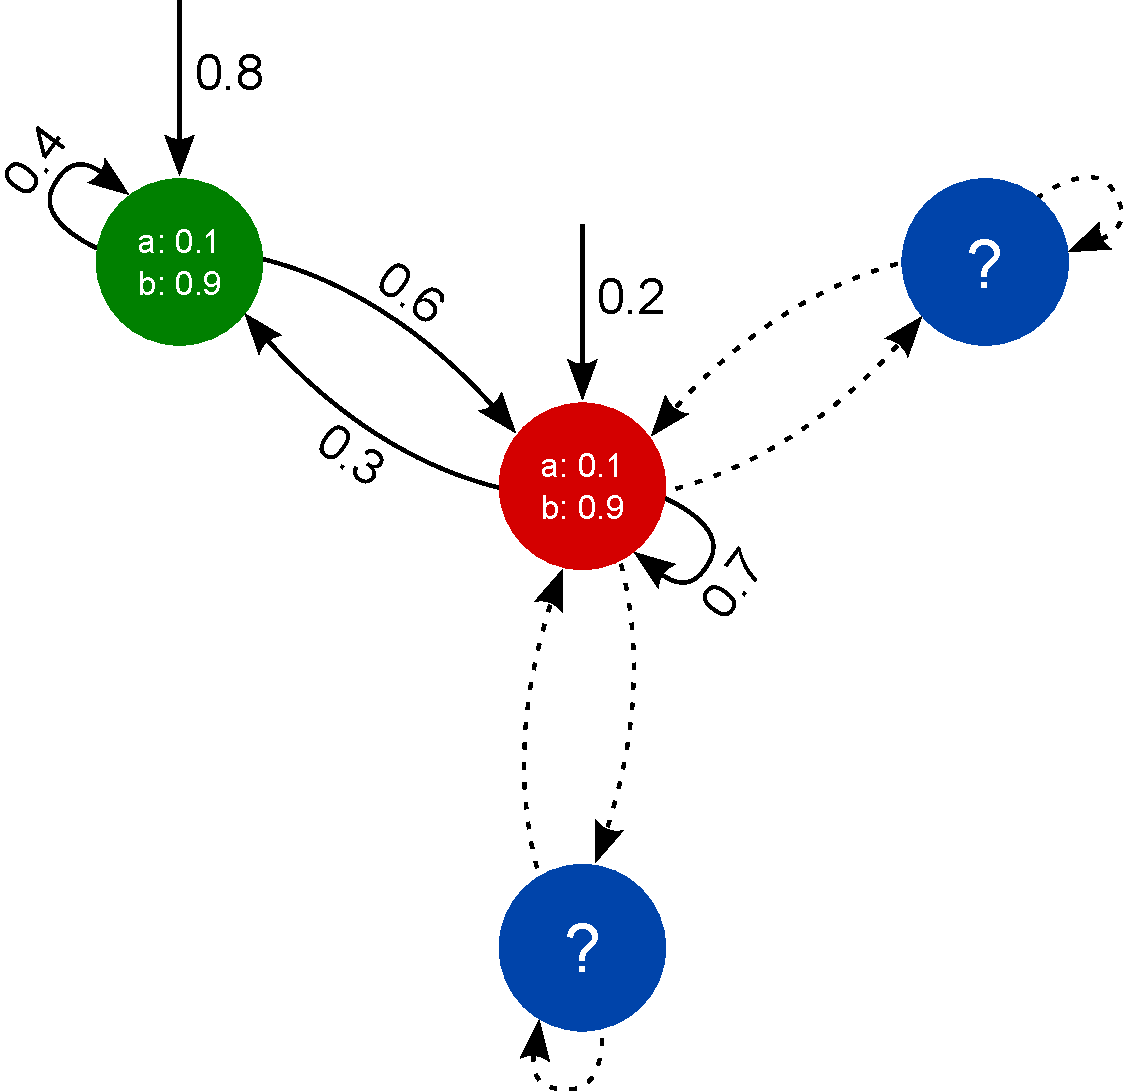
\includegraphics[width=1\linewidth]{pictures/frontpagemodel.pdf}
			\label{fig:Frontpage}
		\end{figure}
	\end{center}
\end{titlepage}


%\input{./content/certificate.tex}
\vspace{2in}
\begin{abstract}

This report covers the work done at the 1. candidate semester at Aalborg University. The goal of the project was to learn how to model reality through some technology. The report takes it basis from the Pautomac competition, which was an online parameter learning competition, where the goal of the competition was to use probabilistic automata to learn the approximate distribution over strings. This report covers the use of the hidden Markov model (HMM), the forward-backward, Viterbi and Baum-Welch (BW) algorithm. Different approaches for learning model parameters as well as the structure of the HMM. Pautomac delivered 48 data sets for the parameter learning task, where a subset were used to generate 12 experiment, in an attempt to study how BW and new presented algorithms behave across data set, that were generated by probabilistic model with significantly different parameters and structures. The results from the different data sets were overall not clear. Other experiments were done on sparsity of models, which showed a clear benefit from using sparse models when learning under a time constraint.

\end{abstract} 



\pagenumbering{roman} %numbering before main content starts
\tableofcontents
\listoffigures

\newpage
\pagenumbering{arabic} %reset numbering to normal for the main content

\chapter{Introduction}
\section{Content Overview}
This chapter will introduce the project, lay down some guidelines for the focus of the project and present the problem definition.

In Chapter \ref{chap:analysis}, the used theory is presented and described to give the reader knowledge necessary to understand the work done in the remaining chapters.

Chapter \ref{chap:models}, provides description of the algorithms, and reasoning about what properties should be considered key and thus implemented in the algorithms introduced in the project. Hypothesis for how these algorithms should perform on the data is also stated.

Chapter \ref{chap:experiments}, describes the experiment set up, and how the dataset and rules of the experiments were chosen. Next the hypothesis is put to the test and presents experiments to see how the algorithms performs on different datasets and compare to each other.

In Chapter \ref{chap:results}, the result from all the experiments is shown. Tendencies and patterns in the results are analysed.

Chapter \ref{chap:conclusion}, concludes on the project and reflects on which project objectives were achieved, and what could have been done differently to obtain better results.

Chapter \ref{chap:future_work}, reflects on what can be done as the next step and where to look in order to perform better in the experiments.
\section{Motivation}
The development of these models has been motivated by two disadvantages we have encountered while using the \gls{baum-welch}.
The first problem is that \gls{baum-welch} can be quite computationally expensive.

During this project, we have been using two different \gls{baum-welch} implementations. One written in Python, available at the PautomaC website, and another written in C\#, provided by the Accord.NET framework. The latter was definitely the fastest, it has thus been used in all of our tests.

For a 100-state \gls{hmm}, 10 iterations of \gls{baum-welch} on a small subset (5,000 random sequences) of the training set 1 from the PautomaC website took 510 seconds on an Intel Core i7-4500U. We have seen that converging with a threshold of 0.01 takes about 300 iterations on a training set of 5,000 sequences. Since the complexity of \gls{baum-welch} scales linearly with the number of sequences and iterations, training on a set of 100,000 sequences with 300 iterations would take about $306,000$ seconds, which is about $3.5$ days. And that is still a lower bound estimate considering that more iterations are typically required to converge when learning larger sets of data.

Since the \gls{baum-welch} considers all possible transitions from one state to another, we might be able to decrease its running time if we can lower the number of transitions between states. As we argued in section \ref{sec:hmm-and-sparsity}, real world problems can be well modeled with a \gls{hmm} with a sparse transition matrix.
The second property of \gls{baum-welch} we hope to improve is the requirement for the number of states to be used to be specified up front.
We think a better approach could be to use a small graph initially, then iteratively extend it based on some heuristics.

To summarize, the properties we are looking for in an algorithm is the ability to extend a small initial graph, but doing so in a way that keeps it sparse while still producing good results.
\subsection{Probabilistic automata}
There exist many different automata for learning observations. A general feature of these automatas is that the better an automata can model observations, the harder it will be to train that automata. The best known automatas are the \gls{hmm} and \gls{pfa}, where this report will focus on the use of \gls{hmm}.\cite{pautomacTR}
Other candidates were concidered for this work, including n-gram, Markov chains and some deterministic counterparts to the \gls{pfa}, however all of these are strictly less powerful than the \gls{pfa}. The \gls{hmm} is known to be equivalent with the \gls{pfa}, which of course makes them equally strong in terms of their modelling power.

Other potential candidates include \gls{pcfg} and \gls{ma}, where the \gls{pcfg} shows strength in bio-informatics and \gls{ma} is known to be stronger than the \gls{pfa}. However as mentioned in section \ref{sec:pautomac} the automatas used to produced the data sets are: \gls{mc}, \gls{dpfa}, \gls{hmm} and \gls{pfa}, where modelling strength beyond \gls{pfa} is not necessary. In practice the \gls{pcfg} would manage the data sets just fine, as the data is finite. However in reality an observed system might never stop emitting symbols, where a model based on context free grammar would not be suitable. The reason for this is that the grammatical rules of \gls{pcfg} has to reach a terminal before a string is recognized, which cannot happen on an infinite string.
\input{./content/Introduction/PautomaC.tex}
\section{Problem Definition}

With the wide use of the Baum Welch algorithm for learning the parameters of a \gls{hmm}, it is a natural to ask if one can come up with a better algorithm. Initially, a fixed number of states must be specified when using the Baum Welch algorithm.
If one does not know the most suited number of states for the given problem, one may have to either choose a number of states arbitrarily, or perform tests using different number of states. If time is critical, the latter choice may not be possible. Therefore, an algorithm hopefully exists that eliminates the initial choice of states.
The many data sets and solutions published during the Pautomac competition makes it easy to evaluate the performance of different algorithms.
This naturally leads to our problem definition:



\begin{itemize}
\item \textbf{Problem:}
	\begin{itemize}
	\item Can we develop an algorithm for learning the parameters of an \gls{hmm}, that performs at least as good as Baum Welch on the Pautomac data sets, but which does not require a fixed number of states to be specified initially?
	\end{itemize}
\end{itemize}

%\input{./content/Theory/theory.tex}
\chapter{Analysis}
\label{chap:analysis}
\section{Hidden Markov Models}
\label{sec:hmm}
\glspl{hmm} are one of the most widely used and best known variants of probabilistic finite automata~\cite{pautomacTR, Rabiner89hmm}. The theoretical basis for \glspl{hmm} and associated methods and algorithms were first described in a series of works by L. E. Baum~et~al.~\cite{baum1966, baum1967, baum1968, baum1970, baum1972}.

One can view an \gls{hmm} as an extension of a standard Markov chain. A Markov chain based model has the property that every observed symbol corresponds directly to an associated state of the model. This property is too restrictive for numerous problems. \glspl{hmm} therefore introduce the concept of hidden (unobservable) states with a probability distribution over the observable symbols. The generated symbol thus becomes a probabilistic function of the current hidden state. This extension allows application of \glspl{hmm} to a much larger variety of problems, however also poses new complications, such as increased complexity of evaluation of probability of a given signal (sequence of observable symbols), determining the optimal sequence of hidden states for a given signal or estimation of parameters for the model~\cite{Rabiner89hmm}.

To better illustrate the mechanics behind the \gls{hmm} we provide a simple example. Consider a lottery game with several urns filled with balls of different colours. Every urn may hold different number of balls of a certain colour, or may not even contain balls of some colours at all. In every turn an unbiased arbiter selects one urn randomly (but possibly abiding to some rules given by the urn selected previously) and takes out a random ball out of the selected urn. You are then shown the colour of the ball, not however, from which urn it was taken. The ball is then returned to the appropriate urn and the game continues so forth your goal being to predict the colours that come next. In this simple case, you can observe a sequence of symbols - colours generated by what can be viewed as an \gls{hmm}, where the urns are the hidden states and the observable symbol probability distribution for every urn (state) is given by the colours of the balls inside.

More formally, a finite discrete \acrlong{hmm} with $n \in \mathbb{N}$ (hidden) states $S = \{S_1, S_2, ..., S_n\}$ over an alphabet of $m \in \mathbb{N}$ observable symbols $\Sigma=\{\sigma_1, \sigma_2, ..., \sigma_m\}$ is a tuple: $$\lambda = (\mathbf{A}, \mathbf{B}, \boldsymbol{\pi})$$
Where:
\begin{itemize}
	\item[$\mathbf{A}$] is an $n$ times $n$ square matrix such that an element of the matrix ${a_{ij} \in [0, 1]}$ represents the transition probability from state $S_i$ to state $S_j$. Naturally this implies ${\forall i \in \{1, 2, ..., n\}: \sum_{j=1}^n{a_{ij}} = 1}$.
	\item[$\mathbf{B}$] is an $n$ times $m$ matrix such that an element of the matrix ${b_{ij} \in [0, 1]}$ represents the probability of outputting symbol $\sigma_j$ in state $S_i$. Naturally this implies ${\forall i \in \{1, 2, ..., n\}: \sum_{j=1}^m{b_{ij}} = 1}$.
	\item[$\boldsymbol{\pi}$] is a vector of $n$ variables, ${\boldsymbol{\pi}=(\pi_1, ..., \pi_n) \in [0, 1]^n}$. Where the value $\pi_i$ represents the probability of state $S_i$ being the initial state. Naturally this implies ${\sum_{i=1}^n{\pi_i} = 1}$
\end{itemize}

Such an \gls{hmm} can be used to generate a sequence of observable symbols (signal): $$\mathbf{O} = (o_1, ..., o_T)$$
Where ${\forall t \in \{1, ..., T\}: o_t \in \Sigma}$, $o_t$ is the symbol observed at time $t$ and $T$ is the number of discrete time steps during the observation (number of observed symbols).

Similarly, we denote a sequence of hidden states of the hidden Markov model as: $$\mathbf{Q} = (q_1, ..., q_T)$$
Where ${\forall t \in \{1, ..., T\}: q_t \in S}$, $q_t$ is the state of the model at time $t$ and $T$ is the number of visited states.
We define the probability of the hidden state sequence (walk) $\mathbf{Q}$ given the model $\lambda$ as:
$$P(\mathbf{Q}|\lambda) = \pi_{q_1}a_{q_1q_2}...a_{q_{T-1}q_T}$$

Any signal $\mathbf{O}$ generated by the \gls{hmm} has a corresponding sequence of hidden states $\mathbf{Q}$ the model visited during the generation of the same length. This sequence is typically unknown for modeled real world signals and generally numerous different hidden state sequences may generate the observed signal with different probabilities. We denote the probability of model $\lambda$ producing the observation sequence $\mathbf{O}$ by hidden state sequence $\mathbf{Q}$ as:
$$P(\mathbf{O}|\mathbf{Q},\lambda) = b_{q_1}(o_1)b_{q_2}(o_2)b_{q_T}(o_T)$$

In the above probability definitions we use more lenient notation for simplicity. As the use of this notation is preserved throughout the following sections alongside the notation from definition of the \gls{hmm}. We define it formally for clarity:
\begin{itemize}
	\item[] $a_{S_iS_j}$ where $S_i, S_j\in S$ is used to refer to the value of $a_{ij}$.
	\item[] $\pi_{S_i}$ where $S_i\in S$ is used to refer to the value of $\pi_i$.
	\item[] $b_{S_i}(\sigma_j)$ where $S_i\in S$ and $\sigma_j\in \Sigma$ is used to refer to the value of $b_{ij}$.
\end{itemize}

Furthermore let us define the set of all possible walks through hidden state space of model $\lambda$ of length $T$ as $\mathcal{Q}_\lambda^T$. Thus the probability of model $\lambda$ generating the signal $\mathbf{O}$ can be easily defined as a sum of probabilities of generating the given signal through all hidden state walks weighted by probabilities of the particular hidden state walks: 

\begin{align*}
P(\mathbf{O}|\lambda)&=\sum_{\mathbf{Q}\in\mathcal{Q}^T_\lambda}{P(\mathbf{O}|\mathbf{Q},\lambda)P(\mathbf{Q}|\lambda)}\\
&=\sum_{\mathbf{Q}\in\mathcal{Q}^T_\lambda}{\pi_{q_1}b_{q_1}(o_1)a_{q_1q_2}b_{q_2}(o_2)...a_{q_{T-1}q_T}b_{q_T}(o_T)}
\end{align*}

It should be noted that the \gls{hmm} defined here is finite in the sense of both $n$ and $m$ being finite numbers. An extension to the model allowing infinite number of states, symbols or both is rather straightforward, however we will not be needing this extension for the purposes of this publication and thus it will be omitted.

\subsection{Hidden Markov Model Evaluation}
It is meaningful and desirable to evaluate a model once constructed and learned. Such evaluation is usually done by computing the probability of the model producing a certain observation sequence. Therefore for a model $\lambda = (\mathbf{A}, \mathbf{B}, \boldsymbol{\pi})$ and a (test) sequence $\mathbf{O}$, we want to compute $P(\mathbf{O}|\lambda)$. Going by the definition one arrives at a summation over all possible walks through hidden state space of model $\lambda$ of length $T$. It is simple to see that, with the presumption that the model is unrestricted (i.e., matrix $\mathbf{A}$ is dense), there is exponentially many of such walks in terms of their length $T$ ($|\mathcal{Q}_\lambda^T|\in\mathcal{O}(N^T)$). Computing the given summation and thereafter computing $P(\mathbf{O}|\lambda)$ by definition is computationally infeasible.

Luckily, an iterative dynamic programming approach exists that can help us compute the coveted probability, called the \gls{fb_algorithm}~\cite{baum1967, baum1968}. The \gls{fb_algorithm} is composed of computing two separate sets of variables (forward and backward), both of which can be used to compute the probability $P(\mathbf{O}|\lambda)$.

The forward variable $\alpha_t(i)$, formally defined as: $$\alpha_t(i)=P((o_1, ..., o_t), q_t=S_i|\lambda)$$ describes the probability that we observe the first $t$ symbols of the given signal and end in the state $S_i$ at the time $t$ given the model $\lambda$.

The forward variable can be computed iteratively as:
\begin{align*}
\forall i\in \{1, ..., n\}&: \alpha_1(i)=\pi_ib_{S_i}(o_1)\\
\forall i\in \{1, ..., n\}, t\in\{2, ..., T\}&: \alpha_t(i) = \sum_{j=1}^n{(\alpha_{t-1}(j)a_{ji})}b_{S_i}(o_t)
\end{align*}

It is easy to see that the probability of an observable sequence $\mathbf{O}$ can be obtained by summing through the forward variables at time $T$ for all of the hidden states:
\begin{align*}
P(\mathbf{O}|\lambda) &= \sum_{i=1}^n{P(\mathbf{O}, q_T=S_i|\lambda)}\\
&= \sum_{i=1}^n{\alpha_T(i)}
\end{align*}

Analogically, the backward variable $\beta_t(i)$, formally defined as: $$\beta_t(i)=P((o_{t+1}, ..., o_T)| q_t=S_i, \lambda)$$ describes the probability that we observe the last $(T-t+1)$ symbols of signal $\mathbf{O}$ given we start at state $S_i$ at the time $t$ and the model $\lambda$.

Again, computing the backward variable is possible iteratively:
\begin{align*}
\forall i\in \{1, ..., n\}&:\beta_T(i)=1\\
\forall i\in\{1, ..., n\}, t\in\{1, ..., T-1\}&:\beta_t(i)=\sum_{j=1}^n{(a_{ij}b_{S_j}(o_{t+1})\beta_{t+1}(j))}
\end{align*}

Once again we straightforwardly obtain a simple way of computing $P(\mathbf{O}|\lambda)$:
\begin{align*}
P(\mathbf{O}|\lambda) &= \sum_{i=1}^n{P(\mathbf{O}|q_1=S_i, \lambda)}\\
&= \sum_{i=1}^n{\beta_1(i)}
\end{align*}

After a careful observation one can see that both approaches, using forward or backward variables, give as an efficient way to compute $P(\mathbf{O}|\lambda)$ in complexity $\mathcal{O}(Tn^2)$~\cite{Rabiner89hmm}.

\subsection{Optimal Hidden State Sequence}

It may be useful to determine the hidden state sequence the model used to generate a given observable signal. Which hidden state sequence is optimal is heavily dependent on the optimality criterion. Multiple optimality criteria exist and are meaningful to use for some applications. The most widely used optimality criterion maximises the probability of the whole walk through the hidden state space given the model $\lambda$ and the observable sequence $\mathbf{O}$~\cite{Rabiner89hmm}:
$$\max_{\mathbf{Q}\in\mathcal{Q}_T^\lambda}(P(\mathbf{Q}|\mathbf{O}, \lambda))$$

An algorithmic solution exists for optimisation of maximisation of $P(\mathbf{O}, \mathbf{Q}|\lambda)$, equivalent to the above expression, based on dynamic programing methods, called \gls{viterbi}~\cite{Viterbi1967, Forney1973}. The algorithm iteratively computes the best single state path score for the first $t$ symbols of the observed sequence. We denote this score for state $i$ and time $t$ as $\delta_t(i)$:
$$\delta_t(i) = \max_{q_1, ..., q_{t-1}}(P((o_1, ..., o_t), (q_1, ..., q_{t-1}), q_t=S_i|\lambda))$$

The $\delta$ variables may be computed iteratively as:
$$\delta_{t+1}(i)=\max_{j\in\{1,...,n\}}(\delta_t(j)a_{ji})b_{S_i}(o_{t+1})$$

Furthermore we define the $\psi$ variable to denote the state for which the iterative computation of the $\delta$ variable is maximised:
$$\psi_{t}(i) = \argmax_{j\in\{1,...,n\}}(\delta_{t-1}(j)a_{ji})$$

The $\psi$ variable serves the purpose of remembering for which states was the score maximised and is necessary for backtracking the optimal sequence.

The \gls{viterbi} itself can be illustrated in four simple steps:
\begin{align*}
	\intertext{Step 1 - Initialisation}
		\forall i\in\{1,...,n\}: \delta_1(i) 	&= \pi_ib_i(o_1)\\
		\forall i\in\{1,...,n\}: \psi_1(i) 	&= 0
	\intertext{Step 2 - Recursion}
		\forall i\in\{1,...,n\},\forall t\in\{2,...,T\}: \delta_t(i)	&= \max_{j\in\{1,...,n\}}(\delta_{t-1}(j)a_{ji})b_i(o_t)\\
		\forall i\in\{1,...,n\},\forall t\in\{2,...,T\}: \psi_t(j) &= \argmax_{j\in\{1,...,n\}}(\delta_{t-1}(j)a_{ji})
	\intertext{Step 3 - Termination}
		p &= \max_{i\in\{1,...,n\}}(\delta_T(i))\\
		q_T &= \argmax_{i\in\{1,...,n\}}(\delta_T(i))
	\intertext{Step 4 - Optimal walk (hidden state sequence) backtracking}
		\forall t\in\{T-1,...,1\}: q_t &= \psi_{t+1}(q_{t+1})
\end{align*}

The determined optimal sequence is thus $\mathbf{Q}=(q_1,...,q_T)$ and the probability of the signal $\mathbf{O}$ being generated by the determined sequence $\mathbf{Q}$ given the model $\lambda$ is stored in the variable $p = P(\mathbf{O},\mathbf{Q}|\lambda)$.

%The \gls{viterbi} is briefly illustrated by the following pseudocode:
%\begin{lstlisting}[mathescape=true]
%real, int[] Viterbi (int n, int T, real[,] A,
% real[,] B, real[] $\pi$, int[] O) begin
%   real[,] $\delta$ := new real[T,n] //$\delta$[t,i] = $\delta_t(i)$
%   int[,] $\psi$ := new int[T,n] //For backtracking
%   real p := 0.0 //Best score
%   int[] q := new int[T] //Optimal sequence
%   
%   //Initialisation
%   for int i := 1 to n do begin
%      $\delta$[1,i] := $\pi$[i]B[i,O[1]]
%      $\psi$[1,i] := 0
%   end
%   
%   //Iteration
%   for int t := 2 to T do begin
%      for int j := 1 to n do begin
%         $\delta$[t,j] := 0
%         for int i := 1 to n do begin //Maximum over i
%            if $\delta$[t,j] < $\delta$[(t - 1),i]A[i,j]B[j,O[t]] then
%             do begin
%               $\delta$[t,j] := $\delta$[(t - 1),i]A[i,j]B[j,O[t]]
%               $\psi$[t,j] := i
%            end
%         end
%      end
%   end
%   
%   //Termination
%   for int i := 1 to n do begin //Maximum over i
%      if p < $\delta$[T,i] then do begin
%         p := $\delta$[T,i]
%         q[T] := i
%      end
%   end
%   
%   //Backtracking
%   for int t := (T - 1) downto 1 do
%      q[t] := $\psi$[(t + 1), q[t + 1]]
%
%   return p, q;
%end
%\end{lstlisting}

\subsection{Estimating Model Parameters}
\label{sec:baum-welch}
There is no analytical solution known for finding model parameters $\mathbf{A}$, $\mathbf{B}$ and $\boldsymbol{\pi}$ maximising the probability of a given observable sequence. In fact, no optimal way to estimate the parameters for \glspl{hmm} exists. However, an iterative method, the \gls{baum-welch}~\cite{baum1970}, can be used to derive $\lambda = (\mathbf{A}, \mathbf{B}, \boldsymbol{\pi})$ such that $P(\mathbf{O}|\lambda)$ is locally maximised for a given signal $\mathbf{O}$. The \gls{baum-welch} has been shown to be equivalent to the \gls{em} method for \glspl{hmm}~\cite{Dempster1977, wu1983}.

In this section we present a simple iterative approach to estimation of \gls{hmm} parameters based primarily on the \gls{baum-welch}. This approach works for a single observable symbol sequence, however the \gls{baum-welch} can be extended to account for train data composed of multitude of signals~\cite{Rabiner89hmm, levinson1983, li2000}.

We first define a couple of auxiliary variables to simplify the consequent constructs:

\begin{align*}
\forall t\in\{1,...,T-1\},\forall i,j\in \{1,...,n\}: \xi_t(i,j) &= P(q_t =S_i, q_{t+1}=S_j|\mathbf{O},\lambda)\\
&= \frac{\alpha_t(i)a_{ij}b_{S_j}(o_{t+1})\beta_{t+1}(j)}{\sum_{k=1}^n\sum_{l=1}^n(\alpha_t(k)a_{kl}b_{S_l}(o_{t+1})\beta_{t+1}(l))}\\
\\
\forall t\in\{1,...,T-1\},\forall i\in\{1,...,n\}: \gamma_t(i) &=P(q_t=S_i|\mathbf{O},\lambda)\\
&=\sum_{j=1}^n\xi_t(i,j)\\
\forall i\in\{1,...,n\}: \gamma_T(i) &= P(q_T=S_i|\mathbf{O},\lambda)\\
&= \frac{\alpha_T(i)}{\sum_{j=1}^n\alpha_T(j)}
\end{align*}

Where the variable $\xi_t(i,j)$ equals the probability of being in state $S_i$ at the time $t$ and transitioning to state $S_j$ at time $(t+1)$ given the model $\lambda$ and observable sequence $\mathbf{O}$. The variable $\gamma_t(i)$ equals the probability of being in state $S_i$ at time $t$.

Given some model $\lambda = (\mathbf{A},\mathbf{B},\boldsymbol{\pi})$, possibly with completely random parameters, we can then iteratively compute a new model $\overline{\lambda} = (\mathbf{\overline{A}},\mathbf{\overline{B}},\boldsymbol{\overline{\pi}})$ as:

\begin{align*}
\forall i\in\{1,...,n\}: \overline{\pi_i} &= \gamma_1(i)\\
\forall i,j\in\{1,...,n\}: \overline{a_{ij}} &= \frac{\sum_{t=1}^T\xi_t(i,j)}{\sum_{t=1}^{T-1}\sum_{k=1}^n\xi_t(i,k)}\\
\forall i\in\{1,...,n\},\forall j\in\{1,...,m\}:\overline{b_{ij}}&=\frac{\sum_{t\in\mathcal{T}_\mathbf{O}(\sigma_j)}\gamma_t(i)}{\sum_{t=1}^T\gamma_t(i)}
\end{align*}

Where for $\sigma \in \Sigma$ and signal $\mathbf{O}$, $\mathcal{T}_\mathbf{O}(\sigma) = \{t\in\{1,...,T\}|o_t=\sigma\}$

\begin{samepage}

In simpler terms:
\begin{itemize}
\item[$\overline{\pi_i}$] is the expected number of times state $S_i$ is visited at time $1$. The property $\sum_{i=1}^n\overline{\pi_i}=1$ is satisfied automatically as $\sum_{i=1}^n\gamma_1(i)=1$ holds by definition.
\item[$\overline{a_{ij}}$] is the expected number of transitions from state $S_i$ to state $S_j$, normalised by expected number of all transitions from state $S_i$ in order for the property $\sum_{j=1}^n\overline{a_{ij}}=1$ to be satisfied.
\item[$\overline{b_{ij}}$] is the expected number of times state $S_i$ is visited and the symbol $\sigma_j$ is outputted simultaneously. Again, a normalisation by expected number of times in state $S_i$ is required to satisfy the property $\sum_{j=1}^m\overline{b_{ij}}=1$.
\end{itemize}
\end{samepage}

The above definition can be obtained from standard Lagrange optimisation using Lagrange multipliers for the maximisation of the Baum auxiliary function~\cite{Rabiner89hmm}:
$$Q(\lambda,\overline{\lambda})=\sum_{\mathbf{Q}\in\mathcal{Q}^T_\lambda}(P(\mathbf{Q}|\mathbf{O},\lambda)\log(P(\mathbf{O},\mathbf{Q}|\overline{\lambda})))$$

Note that $\mathcal{Q}^T_\lambda = \mathcal{Q}^T_{\overline{\lambda}}$ in the case the afore stated computation of $\overline{\lambda}$ is employed, as $\overline{a_{ij}}=0$ if $a_{ij}=0$.

Baum et al.~\cite{baum1968, baum1970, baker1975} have proven that the maximisation of the above expression leads to higher probability of outputting the coveted signal $O$:
$$\overline{\lambda}=\max_{\lambda'}{Q(\lambda,\lambda')} \rightarrow P(\mathbf{O}|\overline{\lambda}) \geq P(\mathbf{O}|\lambda)$$

Moreover the convergence of this method has also been proven by Baum et al.~\cite{baum1968, baker1975}. Namely a model $\overline{\lambda}$ computed by the previously given definition is either:
\begin{enumerate}
\item a critical point of probability function $P(\mathbf{O}|\lambda)$ implying that $\overline{\lambda}=\lambda$.
\item a model with higher probability of producing the desired observable sequence $\mathbf{O}$, meaning $P(\mathbf{O}|\overline{\lambda}) > P(\mathbf{O}|\lambda)$
\end{enumerate}

The whole \gls{baum-welch} can also be viewed as an instance of an \gls{em} algorithm. In this case the computation of the Baum auxiliary function ($Q(\lambda,\overline{\lambda})$) would be the expectation (E) step, whilst the maximisation (M) step would be maximisation over the values of $\overline{\lambda}$~\cite{Dempster1977, Rabiner89hmm}.

As learning the \gls{hmm} parameters can be considered an optimisation problem, other approaches are possible, such as the gradient techniques~\cite{levinson1983, Rabiner89hmm}.

\subsection{Variations}

In general case, the \gls{hmm} as defined would be ergodic - between each couple of states, there exists a finite path with non-zero probability. For many applications it is desirable to restrict the model in some fashion. The most commonly known of such restrictions is the so called left-right model also known as the Bakis model. This model only allows transitions in the hidden state space in one direction, formally: $$\forall i,j \in \{1, ..., n\}; i < j: a_{ji} = 0$$
The left-right model is used extensively for speech recognition.~\cite{bakis1976, jelinek1976}.

The \gls{hmm} considered here follows the standard definition where the observable symbol is outputted in a state of the model. A modification is possible and used, again in the field of speech recognition, in which the outputted observable symbol is associated with a transition instead of a state~\cite{Rabiner89hmm, jelinek1983}. It has been proven useful to incorporate transitions that output no symbol (null transitions) into this modification~\cite{jelinek1983}.

The \gls{hmm} defined in this section is a discrete \acrlong{hmm}, with both discrete probability distribution of the observable symbols as well as a discrete distribution of transition probabilities on hidden states. It is possible to generalise an \gls{hmm} by changing both of the afore mentioned probability distributions into continuous ones. Typically the Gaussian distribution is used~\cite{cappe2005, piyathilaka2013}. In general case however, exact inference is infeasible in \glspl{hmm} with continuous latent variables and approximation methods must be used (extended Kalman filter, particle filter)~\cite{cappe2005}.

As was mentioned before, the definition we presented is for a finite model but can be extended to account for infinite number of states or observable symbols straightforwardly. Many other variants, modifications and extensions also exist, some of them hinted in~\cite{Rabiner89hmm}.

	\subsection{Similarity with Probabilistic Automatons}
The Pautomac competition data has been generated by \gls{pa}s. Since we are concerned with the problem of learning the parameters of a \gls{hmm} that best describes the training data we are given, we need to reason about the difference between \gls{hmm}s and probabilistic automatons. The \gls{pa} is more or less equivalent to the \gls{hmm} in the way it works. Each state in a \gls{hmm} has a probability of emitting a given symbol, while the \gls{pa} defines these emission probabilities as a label on the transitions between states\cite{pautomacTR}. This difference does however still allow for converting back and forth between the two models.
A more significant difference is the \gls{pa}'s use of halting probabilities, which for each state defines the probability of halting immediately after transitioning to that state. Because of the halting probabilities, the \gls{pa} generates of strings of finite length, as long as we assume that all states can reach a state that has a halting probability greater than 0. In contrast to the \gls{pa}, the \gls{hmm} does not have halting probabilities. Thus, the \gls{hmm} generates infinite sequences. However, the \gls{hmm} can easily be modified to include halting probabilities, just as the \gls{pa} can be modified to discard the halting probabilities. In both ways, we get two equivalent models.

In \ref{fig:model-with-and-without-stop-symbols}, the model to the left is a \gls{pa}, and the model to the right is a \gls{hmm}.
Notice that for the \gls{pa}, the probability of stopping when entering the state A is written inside the circle.

\begin{figure}
\begin{centering}
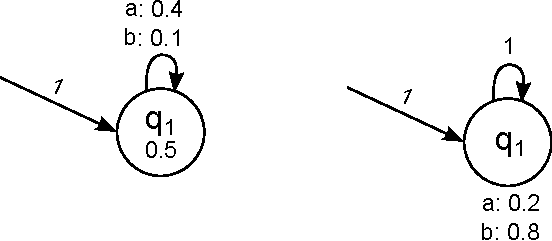
\includegraphics[scale=1]{./pictures/model-with-and-without-stop-symbols.pdf}
\label{fig:model-with-and-without-stop-symbols}
\caption{A \gls{pa} and \gls{hmm}.}
\end{centering}
\end{figure}

We will now consider the probability distributions both models define, to see what impact is has, that only the \gls{pa} defines a halting probability.
With the \gls{pa}, we can calculate the probability of generating an empty sequence, simply by starting in state 1 and stopping immediately before emitting any symbols. That is, $P_{PA}(\varepsilon) = 0.5$. We can of course also produce non empty sequences. For instance, we have that $P_{PA}(a) = \pi_1\phi_{1,a,1}F_1 = 0.2$, where $\pi_q$ is the probability of starting in state $q$, $F_q$ is the probability of stopping right after entering state $q$, $\phi_{q,s,q'}$ is the probability of going from state $q$ to state $q'$ while emitting the symbol $s$.
In the same manner, we get that $P_{PA}(b) = 0.05$.
If we in this way calculate a probability for all possible sequences, we will see that all of those probabilities sum to 1. Thus, the \gls{pa} defines a probability distribution over $\Sigma^\ast$\cite{Dupont:2005:LPA:1746577.1746601}.

When we turn our look to the \gls{hmm}, we see that its structure looks very much like the structure of a \gls{PFA]}.

Without stop probabilities, the probability definition it defines should not be interpreted in the same way as for the \gls{pa}. For instance, it does not make sense to define the probability of the empty sequence $P_{hmm}(\varepsilon)$. Also, if we start to calculate the probabilities of particular sequences in the straight forward way, we get that $P_{HMM}(a) = 0.2$, $P_{HMM}(b) = 0.8$. It is easy to see, that the missing stop probabilities causes the following property to hold:

\[\forall n, \sum_{w \in \Sigma^n} P(w) = 1\]

This means, that in contrast to the \gls{pa}, the \gls{hmm} defines a probability distribution over $\Sigma^n, \forall n \in \mathbb{N}$\cite{Dupont:2005:LPA:1746577.1746601}.

The test data of the Pautomac competation should be assigned probabilities according to a distribution over $\Sigma^\star$.
This is both stated on the Pautomac website, but could also be determined from the fact that the test set contains empty sequences. However, some small modifications allow the \gls{hmm} to behave equivalent to the \gls{pa}, in terms of defining a probability distribution over $\Sigma^\ast$. One way is to add a new symbol $x$ to $\Sigma$, which should be interpreted as a stop symbol. The symbol $x$ is then added to the end of all sequences, including the empty sequence. Instead of using a stop symbol, one could also add a single final state with no emission probabilities and no out transitions.\cite{Dupont:2005:LPA:1746577.1746601}.
\section{HMM and sparsity}
It is our experience that when using a \gls{hmm} to model real world processes, the transition matrix often becomes sparse due to the nature of the process modeled.
For example, in human trait recognition, a \gls{hmm} can be used to model the motion of a particular person while he walks\cite{trait-recognition}.
If focusing on the lower part of the body, consider one state that represents the longest gap between the two feet while walking, where the right foot is in front. It is natural that this state cannot directly lead to the opposite state where the left foot is in front. There has to be a number of intermediate states to represent a more fluid movement, and hence the transition matrix may be quite sparse \gls{hmm}.

When building a system to recognize handwritten text, the transitions matrix of a \gls{hmm} can capture the probability of seeing a particular letter given a letter that precedes it.
In the English language (and possible many other languages), there are many instances of two particular letters, that very rarely or never occur next to each other. An example of the transition probabilities between letters in the English alphabet can be seen in figure \ref{fig:ocr-transitions}, which was made from an analysis of 6020 handwritten words provided by Rob Kassel at MIT Spoken Language Systems Group\cite{thomas-letter-pair-analysis-picture}. Visually, it seems like the transition matrix has many probabilities of zero or very close to. The handouts\cite{leon-letter-pair-analysis-handouts} of Jeffrey S. Leon, confirms the many zero values by providing specific number of occurrences based on analysis of seven English language novels.
\begin{figure}
\includegraphics[scale=0.4]{pictures/ocr-transitions.jpg}
\label{fig:ocr-transitions}
\caption{The transition probabilities between two letters in an English word. White colour denotes a probability of 0 while black denotes a probability of 1.}
\end{figure}
%\section{Other Probabilistic Models}
\subsection{Markov models}

\subsection{n-Gram}
The n-Gram model defines a probability of observing symbol $y$ at time $t$, denoted $y_t$, given the $n-1$ prior symbols. For a 3-gram, also known as a trigram, the probability of producing symbol $s$ is defined as:
\begin{description}
\item $Pr(y_t | y_{t-2}, y_{t-1}) = Pr(y_t, y_{t-1}, y_{t-2}) \frac{1}{|S|}\Sigma_{s \in S} Pr(s_t, s_{t-2}, s_{t-1})$. 
\end{description}
And determining the probability for an observed sequence can then be defined by:
\begin{description}
\item $Pr(y_1, y_2 \dots y_n) = \prod_{t = 1}^{n} Pr(y_t | y_{t-2}, y_{t-1})$ \cite{Notesw4705}
\end{description}
According to \cite{PautomaCTR}, whether n-grams can be consistently outperformed by PFA, HMM or DPFA models for prediction tasks, is still an open problem. n-grams are less powerful than the before mentioned models, however the n-gram’s structure and parameters are easier to compute, which often gives an effective model in practice.

\subsection{Markov Chain}
Markov chains resembles n-grams, as the probability of observing a symbol s at timepoint $t$, $s_t$, is based upon the previous $t-1$ observations $Pr(s_t | s_0, \dots ,s_{t-1})$. However the Markov assumption says that observation $s_t$ is independent from all other observations, except the the single previous observation $s_t-1$:
$$Pr(s_t | s_0, \dots ,s_{t-1}) = Pr(s_t | s_{t-1})$$
This independence assumption stem from the notion that variables after timepoint $t$ can be ignored and variables before timepoint $t-1$ can be eliminated by matrix multiplication, or some variable elimination procedure. \cite{poole2010artificial}

\subsection{Probabilistic Suffix Trees}
\subsection{Deterministic Probabilistic Finite Automata}
\subsection{Probabilistic Residual Finite State Automata}

%\subsection{Probabilistic Finite Automata}
%The \gls{pfa} is a non-deterministic automata with probability modification added to it. The \gls{nfa} consist of:
%\begin{itemize}
%\item A finite set of states $Q$
%\item A finite set of input symbols $\sigma$
%\item A transition function $\f Q  \cprod \sigma \arrow P(Q)$
%\item And a set of accepting states $F$
%\end{itemize}
%
%The NFA’s transition function \f is a probabilistic one and every node have a probability of both starting and accepting the input. The starting and accepting probability is given by an initial and final distribution over the state space. \cite{1966some}


\subsection{Hidden Markov Model}
The hidden Markov model is a special case of the Markov chain model. The HMM models the state transition probabilities just like the Markov chain, but it also models O, which is the set of observation probabilities for each state. In comparison, the Markov chain simply designated a symbol to a single state.
Just like the Markov chain, the state at time t only depends on the previous state at time $t-1$: $Pr(s_t | s_{t-1})$
And the observation at time t only depends on state $s_t$:
\begin{description}
\item $Pr(o_t | s_t)$
\end{description}


Introducing this second layer of probability, simply allows for the model to learn more complex systems, for instance a system where states produce more than one observable symbol. \cite{poole2010artificial}

\subsection{Multiplicity Automata}



%\input{./content/Analysis/pcfgs.tex}
\section{Avoiding Zero Values}

<<<<<<< HEAD
When training a model it is not certain that all possible sequences of symbols are read. Because of this uncertainty there is a chance that some sequences are not given a probability in the model, in other words a zero probability represents that sequence. Also if no measures are taken against it, underflows might happen for very small probabilities. In either cases a zero value will be present in the resulting model. Avoiding these zero values is important, as the zero probability will otherwise be propagated through multiplication, where a single transformation in a sequence with no probability, will mean that the entire sequence has no probability. In the case of PautomaC we evaluate a test by using the normalized probability of 1000 sequences in the perplexity equation. If just one of these sequences has a zero probability the entire test will evaluate to zero probability, even if the other 999 sequences has good probabilities. The reason for this is that the logarithm for a zero valued probability evaluates to minus infinite, which will of course negate the probability of all the other sequences.
=======
When training a model it is not certain that all possible sequences of symbols are read. Because of this uncertainty there is a chance that some sequences is not given a probability in the model, in other words a zero probability represents that sequence. Also if no measures are taken against it, underflows might happen for very small probabilities. In either cases a zero value will be present in the resulting model. Avoiding these zero values is important, as the zero probability will otherwise be propagated through multiplication, where a single transformation in a sequence with no probability, will mean that the entire sequence has no probability. In the case of PautomaC we evaluate a test by using the normalized probability of 1000 sequences in the perplexity equation. If just one of these sequences has a zero probability the entire test will evaluate to zero probability, even if the other 999 sequences has good probabilities. The reason for this is that the logarithm for a zero valued probability evaluates to minus infinite, which will negate the probabilities of all the other sequences.
>>>>>>> 9959f05a769dcce255e6d6997faa3b210f481bf6


One method for avoiding zero values is smoothing. With smoothing the probabilistic weight from the more probable sequences are moved slightly to the less probable ones. This ensures that zero weights will be non existing. Underflows can also be avoided using smoothing, it is however depended on the smoothing technique.


In the case of the PautomaC competition, the test data is available together with the training data. This means that if the models are trained on both the training and test data, smoothing can effectively be avoided, as all possible sequences will be read and given some probability. Underflow is however still an issue, where a negative logarithm representation can be used to ensure that even extremely small probabilities do not underflow.
	

\subsection{Underflow}
    Arithmetic underflow is a condition that can happen in computers, underflow is caused when a number is smaller than the minimum non-negative number a computer can store, and will therefore cause rounding errors bigger than usual. This can be seen by looking at how a computer stores numbers in binary, by looking at a 1 byte binary number with one byte before the decimal point and one byte after we get:\\

\begin{table}[!h]
    \begin{tabular}{|l|l|l|}
        \hline
        Bit number & Value    & Decimal \\ \hline
        3          & $2^3$    & 8       \\ 
        2          & $2^2$    & 4       \\ 
        1          & $2^1$    & 2       \\ 
        0          & $2^0$    & 1       \\ 
        -1         & $2^{-1}$ & 0.500   \\ 
        -2         & $2^{-2}$ & 0.250   \\ 
        -3         & $2^{-3}$ & 0.125   \\ 
        -4         & $2^{-4}$ & 0.0625  \\
        \hline
    \end{tabular}
\end{table}

	\begin{figure}
		\centering
		\includegraphics[width=1\linewidth]{pictures/binary_underflow.png}
		\caption{Binary representation}
		\label{fig:binary_underflow}
	\end{figure}


    This makes the smallest number $0.0625$, any value less than this will get rounded either down to zero or up to $0.0625$. The smallest number in binary is:

    $$0000.0001 = 0.0625$$

\subsubsection{Does it matter}
In many cases underflow could be neglected, if the program is not working with very small numbers, or the accuracy is not that important, but in some cases and for solid programs the program should be able to detect underflow. If an algorithm is working with probabilities and a very small number is inaccurate or zero, computing calculations with this number could cause big problems, especially in cases where the program will try to divide with zero. This is a very important event to be concerned with when working with probabilities that can become very small.  

\subsubsection{How to work around it}
In this project there is a high probability that very small numbers will occur, this demands a work around to the underflow problem. 
\paragraph{Log Odds}
One possible work around is called \textit{log odds} this method maps values $[0;1]$ to $[-\infty; \infty]$. The log odds for a proposition \textit{A} is the logarithm of the probability for proposition $A$ divided by the probability for $\neg A$.\\

    $$\frac{p(A)}{p(\neg A)} = \frac{p(A)}{1-p(A)}$$

    $$l(A) = \log \frac{p(A)}{1-p(A)}$$

    The mapping is shown on the graph below:\\
	\begin{figure}
		\centering
		\includegraphics[width=1\linewidth]{pictures/logodds_mapping.png}
		\caption{Mapping for log odds}
		\label{fig:log_odds}
	\end{figure}

Although \textit{log odds} is a good solution for a lot of problems, there are some situations where
it is not very practical.
One of these situations is when one needs to compute a lot of sums.
Because the sum of two log odds are equivalent to the product of their probabilities, it becomes 
necessary to convert them back into probabilities in order to compute the sum.

\paragraph{Language APIs}
    Another way to work around the problem is by using specific methods available in some programming languages.
     Like with the \textit{decimal} library in Python, this library makes it possible to store decimal numbers with exact precision and detect underflow. 
     It possible to define how many decimals you want on numbers in the decimal library.

\paragraph{Scaling}

Another method for combating underflows is by using a technique called scaling.
Scaling is often used in the baum-welch because the probabilities in the
transition and emission matrices quickly becomes very small.\cite[p.5]{shen2008}

A common way to scale the forward variables in baum-welch is.

\begin{itemize}
\item Initialization
\begin{align*}
\ddot{a}_1(i) &= a_1(i) \\
c_1 &= \frac{1}{\sum_{i=1}^N \ddot{a}_1(i)} \\
{\hat{a}}_1(i) &= c_1 \ddot{a}_1(i)
\end{align*}

\item Induction

\begin{align*}
\ddot{a}_t(i) &= \sum_{j=1}^N \hat{a}_{t-1}(j) a_{ji} b_i(O_t)  \\
c_t &= \frac{1}{\sum_{i=1}^N \ddot{a}_t(i)} \\
{\hat{a}}_t(i) &= c_t \ddot{a}_t(i)
\end{align*}
\end{itemize}

Here we can see that the scaling coefficient $c_t$ at each step only depends on 
the time index t and that the states are summed out.
Also we see that
$$\sum_{i=1}^N \hat{a}_t(i) = 1$$

By induction it can be proven that
$$\hat{a}_t(i) = \bigg(\prod_{\tau=1}^t c_{\tau}\bigg)\alpha_t(i)$$
\cite[p.5]{shen2008}

For backward variables we can use the same scaling factors in each step as for
the forward variables.

\begin{itemize}
\item Initialization

\begin{align*}
\ddot{\beta}_T(i) &= 1 \\
\hat{\beta}_T(i) &= c_T \ddot{\beta}_T(i)
\end{align*}
\item Induction

\begin{align*}
\ddot{\beta}_t(i) &= \sum_{j=1}^N a_{ij}b_j(O_{t+1})\hat{\beta}_{t+1}(j) \\
\hat{\beta}_t(i) &= c_t \ddot{\beta}_t(i)
\end{align*}

\end{itemize}
\cite[p.6]{shen2008}

%
%To determine what method works best, some tests needs to be done, in order to figure out when the \textit{log odds} would be preferable over the \textit{decimal} library.
\subsection{The Overfitting Problem}
When a model is trained and evaluated from data as it is delivered by pautomac, there is a chance of overfitting a model. Overfitting can happen if the set of observations in the training data is not equal to the set of observations in the evaluation data, or in other words if the evaluation data is unseen. The reason for this is simply that if the training data is different from the evaluation data, and the model is perfectly fitted to the training data alone, the unseen evaluation data will fall in probability.

A simple solution to the overfitting problem is to use validation data. Validation data is a secondary training set, that is only used for computing the temporary likelihood for the model while training. Technically the test data from pautomac could be used for validation, but doing so could cause the final evaluation to be less representative of the model's accuracy. The solution that is used for this work, is to split the training set so that at least $\frac{3}{1}$ of the training data is validation data, and at the same time at most $\frac{3}{2}$ of the training data is used for learning a model.
\chapter{Models and Algorithms}
In this chapter, we reason about which properties we think a good algorithm for learning the parameters of a probabilistic automaton should have.
We then propose a number of algorithms that comply to these properties to some extent.

\section{Motivation}
The development of these models has been motivated by two disadvantages we have encountered while using the \gls{baum-welch}.
The first problem is that \gls{baum-welch} can be quite computationally expensive.

During this project, we have been using two different \gls{baum-welch} implementations. One written in Python, available at the PautomaC website, and another written in C\#, provided by the Accord.NET framework. The latter was definitely the fastest, it has thus been used in all of our tests.

For a 100-state \gls{hmm}, 10 iterations of \gls{baum-welch} on a small subset (5,000 random sequences) of the training set 1 from the PautomaC website took 510 seconds on an Intel Core i7-4500U. We have seen that converging with a threshold of 0.01 takes about 300 iterations on a training set of 5,000 sequences. Since the complexity of \gls{baum-welch} scales linearly with the number of sequences and iterations, training on a set of 100,000 sequences with 300 iterations would take about $306,000$ seconds, which is about $3.5$ days. And that is still a lower bound estimate considering that more iterations are typically required to converge when learning larger sets of data.

Since the \gls{baum-welch} considers all possible transitions from one state to another, we might be able to decrease its running time if we can lower the number of transitions between states. As we argued in section \ref{sec:hmm-and-sparsity}, real world problems can be well modeled with a \gls{hmm} with a sparse transition matrix.
The second property of \gls{baum-welch} we hope to improve is the requirement for the number of states to be used to be specified up front.
We think a better approach could be to use a small graph initially, then iteratively extend it based on some heuristics.

To summarize, the properties we are looking for in an algorithm is the ability to extend a small initial graph, but doing so in a way that keeps it sparse while still producing good results.
\subsection{Algorithms}
In this section a number of algorithms are described, which all try to learn the parameters of a \gls{hmm} given a set of training sequences $D$, which contains a number of sequences over $s$ distinct symbols.
In other words, each algorithm will try to find a model that makes the generation of the particular training sequences most likely.
Since a \gls{hmm} can be represented by the use of either matrices or a graph like structure, any of the algorithms may output either a matrix or graph representation of a \gls{hmm}, denoted by $M$ or $G$ respectively.
By $LL(M)$ or $LL(G)$ we denote the likelihood of the training sequences given the model.

The algorithms proposed in this section have been divided into two types.
The static algorithms start with a \gls{hmm} with a particular number of states which will never change.
The dynamic algorithms start with a \gls{hmm} of just a single state, and will dynamically extend the number of states through a number of iterations. 
For the static algorithms, $n$ denotes the number of states to be used.
The dynamic algorithms will by $n$ denote a number of iterations $1, ..., n$, where each iteration extends the model by a single node.
In \ref{fig:alg-hierarchy} the names and classes of our proposed algorithms can be seen. Note that the Baum Welch algorithm has also been included, simply to emphasize which class of algorithms it belongs to. 

\begin{figure}
\label{fig:alg-hierarchy}
\caption{The algorithms used in our experiments}
\Tree[.Algorithms
		[.{Static size} 
			{Baum Welch}
            {Sparse Baum Welch}
        ]
       	[.{Dynamic size} 
       		{Strict George}
       		{George}
       		{Greedy Extend}
      	]
     ]
\end{figure}

Since the Baum Welch algorithm is guaranteed to never worsen $LL(G)$ when run on $G$, it is used internally by some of the algorithms.
By $BW_t(M, D)$ we denote the \gls{hmm} obtained after running Baum Welch on the \gls{hmm} $M$ using the training sequences $D$, and iterating as long as each iteration increases the likelihood by at least $t$.
By $BW^i(M, D)$ we denote the \gls{hmm} obtained after running $i$ iterations of Baum Welch on the \gls{hmm} $M$ using the training sequences $D$.
If a \gls{hmm} is represented by a graph, we denote it $G$, and the similar notations $BW_t(G, D)$ and $BW^i(G, D)$ are used.


\input{./content/Models/Algorithms/greedyextend}
\input{./content/Models/Algorithms/sparsebaumwelch}
\input{./content/Models/Algorithms/statesplitting}
\input{./content/Models/Algorithms/gammastatesplitter}




%\input{./content/work-done/work-done.tex}
\chapter{Experiments}

\section{Choice of Programming Language}
Initially, Python was used for experimenting with the different algorithms (written in Python) which is provided at the Pautomac website. Python is advantageous in the time it takes to create new or alter existing algorithms, as a dynamically typed and very concise language Python provides for quick writing of new code. However, the Python programming language has been found unsuitable for our needs when continuously running multiple benchmarks to measure the performance of new and existing algorithms due to the long run time.

Several attempts to increase the performance of Python were attempted, such as using different interpreters including the standard Python interpreter, Anaconda and PyPy. Different packages claiming to provide fast calculations of floating points of high precision were also tested. In the end, however, the attempted approaches did not provide satisfactory results leading to a switch to C\# programming language achieving the coveted considerable increase in performance.

Alongside the increase in performance, static types used by  C\# have proved to be very convenient when more people have been working on the same code. Unlike Python, the C\# code has achieved much higher level of readability and adequately served as documentation itself. In many cases, we found that we spent much more time documenting our code when using Python.
\section{Test Environment}

To comply with the need to continuously run multiple extensive experiments and test on both newly proposed algorithms and already existing ``baseline'' algorithms a robust test environment framework has been designed and implemented.

Having the test environment framework common for every tested algorithm made it increasingly simple to set up and evaluate the tests and produce extensive result data as a common interface was implemented for every algorithm to feed it training data and obtain the resulting probabilities.

Another important aspect to the test environment is the ability to reuse existing solutions in multiple algorithms. The experimental algorithms we introduce are mainly based around the well known \gls{baum-welch} and thus the test environment may be utilised to provide unified access to the standard \gls{baum-welch} for every of tested approaches, greatly decreasing the code redundancy and allowing for faster creation and testing of new algorithms in the process.

The test environment thus mainly compromises from several main components. The architecture of the test environment and the dependencies and interoperability of the components are depicted in figure \ref{fig:testenvironment}.

\begin{figure}[!htb]
\centering
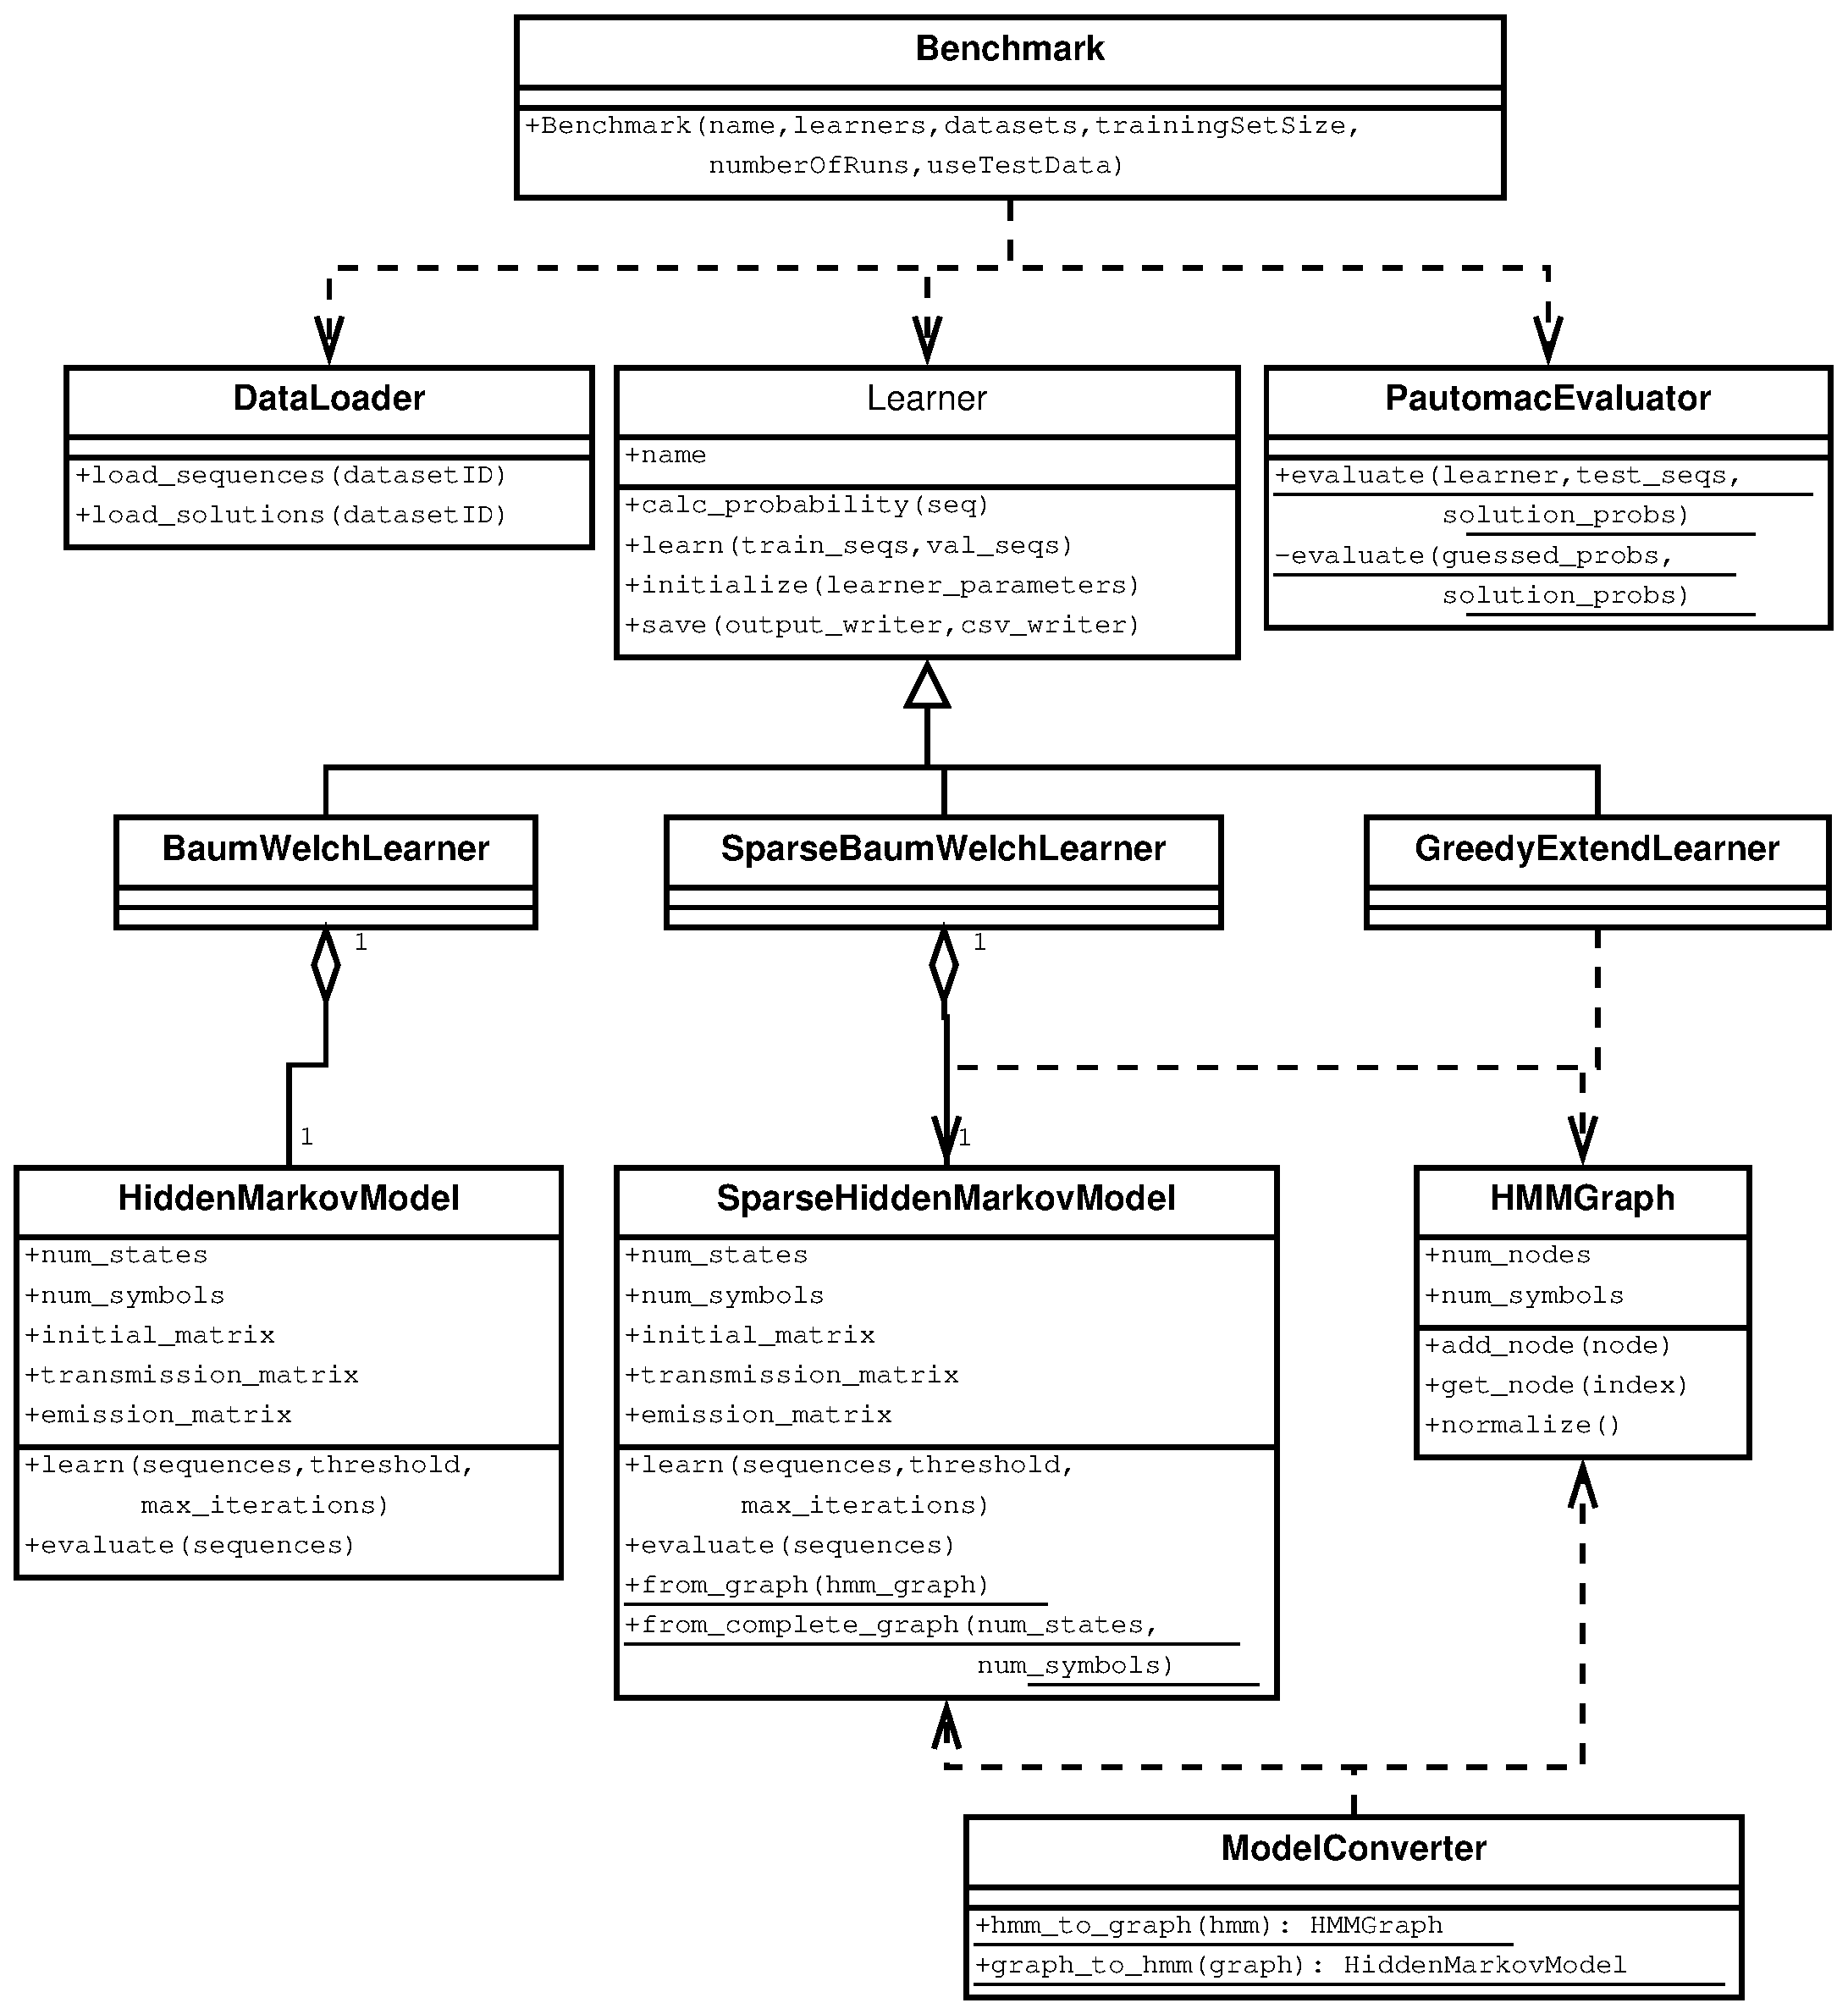
\includegraphics[scale=.4]{pictures/test-environment-overview.eps}
\caption{An overview of the test environment architecture.}
\label{fig:testenvironment}
\end{figure}

\subsection{DataLoader}
The \formatclass{DataLoader} class is responsible for loading both training data, test data and solution data from the files published at the Pautomac website. Both training and test data is represented by a list of sequences, while solution data is represented by a list of probabilities.
This class contains the two functions \formatfunction{load\_probabilities\_from\_file(file\_path)} and \formatfunction{load\_sequences\_from\_file(file\_path)}. The file to be read by both functions must be formatted according to the Pautomac data formats, as described in \todo{insert secref}. The former function outputs a list of sequences, where each sequence is represented by a list of integers.
The latter function outputs a list of probabilities, where each probability is represented by a floating point.

\subsection{Learner}
If one wants to implement a new technique for learning the parameters of a probabilistic model, a new class must be created that derives from the abstract class \formatclass{Learner}.
A learner has only one responsibility: Given a list of training sequences, it must learn a probabilistic model as close as possible to the model used to generate those sequences. How this is done is up to the implementer to choose. The only requirement is that he implements a \formatfunction{calc\_probability(sequence)} function, which given a sequence should return how likely it is that the learned model generated that sequence.
The \formatclass{Learner} class has an already implemented function called \formatfunction{evaluate(sequences, probabilities)}, which uses the \formatfunction{calc\_probability(sequence)} function to calculate probabilities for all provided sequences.
The probabilities are then normalised, and a score is calculated based on the Pautomac evaluation criteria.
The \formatfunction{evaluate} function can be seen by \ref{code:learner}.
A learner should also define a name.

\subsection{Model}
Consider one \formatclass{Learner} that uses the Baum Welch algorithm to estimate the parameters of a Hidden Markov Model and a second \formatclass{Learner} that uses another algorithm, also for estimating the parameters of a Hidden Markov Model. The two learners may need to do many of the same operations on a Hidden Markov Model, e.g. normalization, calculating the probability of being in a particular state or observing a particular sequence at a given time. 
It would be time consuming and increase redundancy if both learners were to implement their own Hidden Markov Model and operations on it.
The \formatclass{Model} has been created to facilitate this. It is an abstract class, which only dictates that a single function must be implemented, which is the \formatfunction{calc\_sequence\_probability(symbol\_sequence)} function. Given a sequence, it must return the probability for the model to generate that sequence. Note that this function is intended to be directly used as the output of the function in the \formatclass{Learner} class having the same name.

\begin{figure}
\caption{The \formatfunction{evaluate} function of the \formatclass{Learner} class.}
\label{code:learner}
\pythonexternal{codeexamples/learner.py}
\end{figure}


\subsection{Evaluator}
This class is responsible for evaluating a \formatclass{Learner} according to the Pautomac evaluation criteria.
Given a learner that has already learned a model, and a number of test sequences with their respective probabilities, it checks how well the probabilities predicted by the \formatclass{Learner} matches the real probabilities.


\subsection{Benchmarker}
For evaluating particular learners on particular data sets, the \formatclass{Benchmarker} class is convenient to use.
As input, it takes a set of learners and data sets, a number of runs, and an output file path.
When run, the \formatclass{Benchmarker} will load all the data sets using the \formatclass{DataLoader}. A data set contains training sequences, test sequences, and a probability associated with each test sequence. For each run, the \formatclass{Benchmarker} randomly splits the training sequences into two sets, where the first $\frac{2}{3}$ sequences are used for training while the remaining are used for validation during training.
Each \formatclass{Learner} will attempt to learn an underlying model for each of the data sets, one by one. When having learned a model for a particular data set, it is evaluated by the \formatclass{Evaluator}. The result of the benchmark is a mean and median score for each pair of learner and data set, which is output to a specified file in .csv format. Besides the mean and median score, the mean and median running time is also measured.
\subsubsection{Sparse Hidden Markov Model}
\label{sec:shmm}

As many of implemented experimental algorithms work with \glspl{hmm} that have sparse transition matrix in the sense of many transition probabilities being zero, we deemed it useful to optimise the algorithms for sparse matrix environment. For this purpose a new model, the \emph{Sparse hidden Markov model}, was implemented to utilise the sparseness of the matrix to achieve increased performance speed compared to standard methods.

The \emph{Sparse hidden Markov model} optimisation is done mainly in the form of storing information on active (non-zero probability) transitions in the model. To achieve this every node remembers all active successors and all active predecessors. This allows the algorithms to only read and compute the values relevant to the underlying \gls{hmm}, thus achieving computational speedup without loss of precision.

The above optimisation build on the property of the \gls{baum-welch} that the probability of a transition will stay as either zero or non-zero (unless an underflow occurs) during iterative update of the parameters.

The above information is utilised by both \gls{baum-welch} and \gls{fb_algorithm}, which is required for evaluation of the model and in the \gls{baum-welch} itself. The \gls{viterbi} was also optimised using the above knowledge. Exhaustive testing has been done to ensure correctness of the algorithm as well as measure the obtained speedup. The tests were conducted using randomly generated dummy data and randomly initialised models. Eight different runs were conducted for every configuration to filter out possible noise. For each run a different random initial configuration was generated and used for both the standard \gls{hmm} and the optimised sparse version. For tests of the \gls{baum-welch} $20$ iterations were conducted for each run for both the standard and sparse versions. The average speedup achieved on either the \gls{baum-welch} or \gls{viterbi} can be seen in graphs \ref{sparseBWspeedup} and \ref{sparseViterbispeedup} respectively.

\begin{figure}
	\centering
	\begin{tikzpicture}
		\begin{axis}[
			width=0.8\textwidth,
			height=0.32\textheight,
			ymin=1,
			ymax=5,
			xlabel = Number of states,
            		ylabel = Average speedup,
            		legend style={at={(0,1)}, anchor=north west}]
			\addplot+table[x=States, y=BW_8, col sep=tab]
			{content/Experiments/graphdata/sparseHMMspeedup10.csv};
			\addlegendentry{A}
			\addplot+table[x=States, y=BW_2, col sep=tab]
			{content/Experiments/graphdata/sparseHMMspeedup10.csv};
			\addlegendentry{B}
			\addplot+table[x=States, y=BW_2, col sep=tab]
			{content/Experiments/graphdata/sparseHMMspeedup5.csv};
			\addlegendentry{C}
		\end{axis}
	\end{tikzpicture}
	\caption{Average speedup achieved on \gls{baum-welch} using the \emph{Sparse hidden Markov model}. \textbf{A:} Tested a model with transition density of 10\% on dummy data with 8 symbols. \textbf{B:} Tested a model with transition density of 10\% on dummy data with 2 symbols. \textbf{C:} Tested a model with transition density of 5\% on dummy data with 2 symbols.}
	\label{sparseBWspeedup}
\end{figure}

\begin{figure}
	\centering
	\begin{tikzpicture}
		\begin{axis}[
			width=0.8\textwidth,
			height=0.32\textheight,
			ymin=10,
			ymax=40,
			xlabel = Number of states,
            		ylabel = Average speedup,
            		legend style={at={(0,1)}, anchor=north west}]
			\addplot+table[x=States, y=VIT_8, col sep=tab]
			{content/Experiments/graphdata/sparseHMMspeedup10.csv};
			\addlegendentry{A}
			\addplot+table[x=States, y=VIT_2, col sep=tab]
			{content/Experiments/graphdata/sparseHMMspeedup10.csv};
			\addlegendentry{B}
			\addplot+table[x=States, y=VIT_2, col sep=tab]
			{content/Experiments/graphdata/sparseHMMspeedup5.csv};
			\addlegendentry{C}
		\end{axis}
	\end{tikzpicture}
	\caption{Average speedup achieved on \gls{viterbi} using the \emph{Sparse hidden Markov model}. \textbf{A:} Tested a model with transition density of 10\% on dummy signal with 8 symbols of length 10000. \textbf{B:} Tested a model with transition density of 10\% on dummy signal with 2 symbols of length 10000. \textbf{C:} Tested a model with transition density of 5\% on dummy signal with 2 symbols of length 10000.}
	\label{sparseViterbispeedup}
\end{figure}

All of the performance tests were coded in C\# programming language just as the rest of the test environment and were solely single threaded. The performance speedup was measured running on a 4-core Intel Core i7-4700MQ processor machine clocked at frequency 2.4 GHz with 8 GB of available \gls{ram} and utilising the Microsoft Windows 8 operating system.

The result graph \ref{sparseBWspeedup} shows that the \gls{baum-welch} speedup using the \emph{Sparse Hidden Markov Model} is largely independent of the number of symbols in the data, however strongly correlated to the negative density (or ``sparsity'') of the model of the transition matrix. The speedup measured for the \gls{baum-welch} achieved a factor of $2.53$ for the 10\%  data density and a factor of $4.72$ for the 5\% density for a $100$ state model. The observed speedup is lower than the expected theoretical value (factor of 10 for 10\% density and 20 for 5\% density). This may be caused by unideal implementation, use of more and more complex data structures and possibly optimisation performed by the compiler.

A significant speedup has been observed for the \gls{viterbi}. As can be observed from the result graph, \ref{sparseViterbispeedup}, the speedup on the \gls{viterbi} is very similar to speedup on \gls{baum-welch}, being independent on the number of symbols and almost linear to sparsity of the model. A speedup by a factor of $20.99$ has been observed for the model with 10\% density, but this factor was increased to $38.01$ with 5\% density model. Both of the discussed results are the highest measured speedups observed for $100$ state models. Contrary to \gls{baum-welch} results, \gls{viterbi} scored better than the expected theoretical speedup.
\section{Selecting Datasets}\label{sec:datasets}
In the PautomaC competition, 48 data sets were used. If we were to conduct experiments on all of those data sets, it would take an unreasonable amount of time.
As a consequence, we have chosen to limit the amount of data sets used in our experiments.
We think the most important parameters that differs between data sets are the number of states used by the generating model, the number of symbols, and the transition density. The number of states and symbols have been published after the competition finished, and the transition density is something we can calculate by examining the models that generated each data set, which was also published when the competition finished.
We define the transition density as the ratio between the number of transitions in the model and the number of states squared (the total number of possible transitions). 

For each of the 3 parameters, 4 data sets have been selected that differ as much as possible on that particular parameter, while the other two parameters differ as little as possible.
Figure \ref{fig:statesetplot} shows how four data sets represent different amount of states, while the number of symbols and transition density almost stay the same. In \ref{density_table} and \ref{symbol_table}, a smilar scatterplot can be seen for the transition density and the number of symbols, respectively.

\begin{figure}
	\centering
	\begin{subfigure}[b]{0.5\textwidth}
        	\begin{tikzpicture}
			\begin{axis}[
			scale = 0.8,
			xlabel = Transition density (\%),
            	ylabel = Number of symbols]
			\addplot[scatter,
				only marks,
				scatter src=explicit] 
				table[meta=mark, x=density, y=symbols, col sep=tab]
				{content/Experiments/graphdata/stateset.csv};
			\end{axis}
		\end{tikzpicture}
        \end{subfigure}%
		\begin{subfigure}[b]{0.5\textwidth}
\begin{tikzpicture}
	\begin{axis}[
	scale = 0.8,
			xlabel = Number of states,
            	ylabel = Number of symbols]
		\addplot[scatter,
			only marks,
			scatter src=explicit] 
		table[meta=mark, x=states, y=symbols, col sep=tab]
		{content/Experiments/graphdata/stateset.csv};
	\end{axis}
\end{tikzpicture}
	\end{subfigure}
  	\caption{Two plots visualising the selected state-range datasets}\label{fig:statesetplot}
\end{figure}

%%%%%%%%%%%%%%%%%%%%%%%
%
%_______density range______________

\begin{figure}
	\centering
	\begin{subfigure}[b]{0.5\textwidth}
        	\begin{tikzpicture}
			\begin{axis}[
			scale = 0.8,
			xlabel = Number of states,
            	ylabel = Number of symbols]
			\addplot[scatter,
				only marks,
				scatter src=explicit] 
				table[meta=mark, x=states, y=symbols, col sep=tab]
				{content/Experiments/graphdata/densityset.csv};
			\end{axis}
		\end{tikzpicture}
		\end{subfigure}%
		\begin{subfigure}[b]{0.5\textwidth}
		\begin{tikzpicture}
	\begin{axis}[
			scale = 0.8,
			xlabel = Transition density(\%),
            	ylabel = Number of symbols]
		\addplot[scatter,
			only marks,
			scatter src=explicit] 
		table[meta=mark, x=density, y=symbols, col sep=tab]
		{content/Experiments/graphdata/densityset.csv};
	\end{axis}
\end{tikzpicture}
\end{subfigure}
  	\caption{Two plots visualising the selected density-range datasets}\label{fig:densitysetplot}
\end{figure}

%%%%%%%%%%%%%%%%%%%%%%%
%
%_______symbol range______________

\begin{figure}
	\centering
	\begin{subfigure}[b]{0.5\textwidth}
        	\begin{tikzpicture}
			\begin{axis}[
			scale = 0.8,
			xlabel = Transition density(\%),
            	ylabel = Number of states]
			\addplot[scatter,
				only marks,
				scatter src=explicit] 
				table[meta=mark, x=density, y=states, col sep=tab]
				{content/Experiments/graphdata/symbolset.csv};
			\end{axis}
		\end{tikzpicture}
       \end{subfigure}%
	\begin{subfigure}[b]{0.5\textwidth}
		\begin{tikzpicture}
			\begin{axis}[
			scale = 0.8,
			xlabel = Number of symbols,
            	ylabel = Number of states]
		\addplot[scatter,
			only marks,
			scatter src=explicit] 
		table[meta=mark, x=symbols, y=states, col sep=tab]
		{content/Experiments/graphdata/symbolset.csv};
	\end{axis}
	\end{tikzpicture}
	\end{subfigure}
  	\caption{Two plots visualising the selected symbol-range datasets}\label{fig:symbolsetplot}
\end{figure}

\FloatBarrier

\begin{table}
\centering
{
\begin{tabular}{| c | c | c | c |}
  \hline
  Dataset 	& \textbf{States} 	& Density (\%) 	& Symbols \\  \hline
  6 			& \textbf{19 }			&	13.5				& 6 \\
  23 			& \textbf{33} 			&	11.4				& 7 \\
  41			& \textbf{54} 			&	14.3				& 7 \\
  1				& \textbf{64} 			&	8.7				& 8 \\ \hline
\end{tabular}
\caption{State amount}
\label{state_table}
}
\end{table}

\begin{table}
\centering
{
\begin{tabular}{| c | c | c | c |}
  \hline
  Dataset 	& States  			& \textbf{Density (\%)} 		& Symbols \\  \hline
  36 			&	54					& \textbf{7.4 }						& 9 \\
  8 			&	49					& \textbf{16.8 }					& 8 \\
  43			&	67					& \textbf{40.2 }					& 5 \\
  37			&	69					& \textbf{54 	}					& 8 \\ \hline
\end{tabular}
\caption{Transition density percentage}
\label{density_table}
}
\end{table}

\begin{table}
\centering
{
\begin{tabular}{| c | c | c | c |}
  \hline
  Dataset 	& States	 	& Density (\%) 	& \textbf{Symbols}	 \\  \hline
  32 			& 43				& 11.8				& \textbf{4}		\\
  8 			& 49				& 16.8 				& \textbf{8}		\\
  10			& 49				& 14.2 				& \textbf{11}	\\
  35			& 47				& 14.2 				& \textbf{20}	\\ \hline
\end{tabular}
\caption{Symbol alphabet size}
\label{symbol_table}

}
\end{table}
\subsection{Experiment Parameters}\label{sec:parameters}

Since the static learners use a \gls{hmm} internally, the number of states used may affect the outcome of the experiments.
The Pautomac models that generated the data sets were generated by at most 73 states, and due to the fact, that the computation effort increases quadratically with the number of states, we deem it unnecessary to test models with more than 100 states. Due to the large amount of time it takes to run the \gls{baum-welch}, a step size of 10 for the number of states tested.
The dynamic learners does not require a specified number of states, as they all start with a model containing just a single state, which in turns are extended.

The data sets given by Pautomac ranges in sequences. Some have 20.000 sequences while others have 100.000. These amounts of sequences are however larger than what is necessary to illustrate how one algorithm behaves, given some dataset. Another problem is that the larger datasets takes significantly longer to compute, compared to a subset of sequences. It is therefore interesting to explore what amount of sequences that will both produces useful results, without spending an unnecessary amount of time doing the computations.

\paragraph{Training Sequences}
The Pautomac training sets contain between 20,000 and 100,000 sequences.
An experiment has been conducted, to see whether all of these sequences are needed to learn a good model using \gls{baum-welch}.
The result is depicted in Figure \ref{fig:sequences}. It seems like it does not improve the result significantly when using more than 100 sequences.
However, it was decided to use 5000 sequences as the running time of \gls{baum-welch} for this amount is still reasonable. It should be noted that the running time increases linearly with the amount of sequences used for training, but quadratically by the number of states, following the complexity of the \gls{fb_algorithm} algorithm.

The setup for this experiment:
\begin{itemize}
\item Dataset: 36
\item Algorithm: Baum Welch
\item Threshold: 0.01
\item Training sequences: 100-50,000
\item Validation sequences: 1,000
\item CPU: 2 Ghz Intel core 2 duo
\end{itemize}

\begin{figure}
	\centering
	\begin{subfigure}[b]{0.5\textwidth}
        \begin{tikzpicture}
		\begin{axis}[
				scale = 0.9,
				ymin = 23000,
				ymax = 24000,
				ybar,
				xtick=data,
   				symbolic x coords={100,500,1000,5000,10000,50000},
				xlabel = Sequences,
            		ylabel = Score (lower is better)]
				\addplot+table[y=score, col sep=tab]
				{content/Experiments/graphdata/sequences.csv};
		\end{axis}%
	\end{tikzpicture}
        \end{subfigure}%
		\begin{subfigure}[b]{0.5\textwidth}
\begin{tikzpicture}
		\begin{axis}[
				scale = 0.9,
				ymin = 0,
				ybar,
				xtick=data,
   				symbolic x coords={100,500,1000,5000,10000,50000},
				xlabel = Sequences,
            		ylabel = Running time (seconds)]
				\addplot+table[y=time, col sep=tab]
				{content/Experiments/graphdata/sequences.csv};
		\end{axis}%
	\end{tikzpicture}
	\end{subfigure}
  	\caption{Plot of Baum-welch score and runningtime on different sequence amounts}\label{fig:sequences}
\end{figure}


\paragraph{Baum-Welch Treshold}
The Baum-Welch algorithm takes two parameters, the amount of states which the trained model should consist of and the threshold of convergence. The state range for the experiments have already been selected to range between 10 and 100 with a step size of 10. Unlike the choice of states, which is a variable, the threshold should be a static value for all the experiments.

Defining the threshold is done by exploring how Baum-Welch behaves on different threshold values. \ref{fig:threshold} shows the results from the experiments. Each threshold parameter value were combined with the parameter of 50 states, and trained on a single dataset.

\begin{figure}
\centering
	\begin{tikzpicture}
		\begin{axis}[
				ybar,
				xtick=data,
   				symbolic x coords={0.1,0.05,0.01,0.005,0.001,0.0001},
				xlabel = Treshold,
            		ylabel = Score (lower is better)]
				\addplot+table[y=Score, col sep=tab]
				{content/Experiments/graphdata/treshold.csv};
		\end{axis}
	\end{tikzpicture}
\caption{Negative logarithmic likelihood when running Baum-Welch with different thresholds.}
\label{fig:threshold}
\end{figure}

Based on the results, it is clear that a threshold of 0.01 will produce useful that are representative for much lower thresholds.

\subsection{Greedy Extend}
10 BW iterations between when after each extend.
100 attempts to extend graph.
0.01 threshold for BW when reaching a maximum of 100 states or if not able to expand further.

Whether we choose to run Greedy Extend a single or multiple times does not seem to have a big impact on the result.
In figure \ref{fig:ge-diversity-5-runs}, the result of 5 different runs of Greedy Extend can be seen. The results of all runs look very similar.
\begin{figure}
\begin{centering}
\begin{tikzpicture}
	\pgfplotsset{every axis legend/.append style={ 
		at={(0.5,1.03)},
		anchor=south}}
	\begin{axis}[
			xlabel = Number of states,
            	ylabel = Score (lower is better),
            	legend columns=-1,
            	legend entries={Run 1, Run 2, Run 3, Run 4, Run 5},
			legend style={/tikz/every even column/.append style={column sep=0.3cm}}]
		
		\addplot+[mark=none]table[x=States, y=Run1, col sep=tab]
		{content/Experiments/graphdata/ge-diversity-5-runs.csv};
		
		\addplot+[mark=none]table[x=States, y=Run2, col sep=tab]
		{content/Experiments/graphdata/ge-diversity-5-runs.csv};
		
		\addplot+[mark=none]table[x=States, y=Run3, col sep=tab]
		{content/Experiments/graphdata/ge-diversity-5-runs.csv};
		
		\addplot+[mark=none]table[x=States, y=Run4, col sep=tab]
		{content/Experiments/graphdata/ge-diversity-5-runs.csv};

		\addplot+[mark=none]table[x=States, y=Run5, col sep=tab]
		{content/Experiments/graphdata/ge-diversity-5-runs.csv};
	\end{axis}
\end{tikzpicture} 
\caption{5 different runs of Greedy Extend on the same data set using $\alpha = 100, \beta = 10$.}
\label{fig:ge-diversity-5-runs} 
\end{centering}
\end{figure}

\chapter{Results}
In the following a number of tests are conducted, to see how the algorithms described in chapter \ref{chap:models}, could have performed in the Pautomac competition. Tests are conducted on the three data sets, 6, 23, and 35. These data sets were chosen according to how well the proposed algorithms in this report performed in comparison to \gls{bw}, such that \gls{bw} seems to loose on data set 6, be quite even on data set 23, and win on data set 35.
The perplexity measure described in section \ref{sec:pautomac} has then been used to evaluate a score.
The parameters chosen for the following tests are all based on the outcome of the experiments described in chapter \ref{chap:experiments}.
For all tests, 5000 sequences from the Pautomac training data files have been used to learn the model. The static algorithms are run with different number of states, starting at 10 with a step size of 10.
The dynamic algorithms are run with 5 intermediate \gls{bw} iterations.
In figure \ref{fig:pautomac-competition-6}, \ref{fig:pautomac-competition-23} and \ref{fig:pautomac-competition-35}, the score on each data set can be seen.
A summary of the best scores on each data set can be seen in table \ref{table:pautomac-best-score}.
The unusual behaviour of \gls{gs} that starts after a number of iterations is expected to be caused by an underflow problem.
One should note that the methods described in section \ref{sec:hmm_vs_pa} that accounts for stop probabilities have not been used for any of the algorithms, which will inevitable cause the score to be worse.


\begin{figure}
\centering
\begin{tikzpicture}
	\pgfplotsset{every axis legend/.append style={
		at={(0.5,1.1)},
		anchor=south}}
	\begin{axis}[
			xmin = 0,
			xmax = 100,
			ymin = 60,
			ymax = 280,
			cycle list name=color list,
			xlabel = States,
            	ylabel = Perplexity (lower is better),
            	legend columns=-1,
            	legend entries={GE, BW, SBW, GS, Goal},
			legend style={/tikz/every even column/.append style={column sep=0.3cm}}]
		
		\addplot+[mark=none]table[x=States, y=GE, col sep=tab]
		{content/Results/pautomac-competition-results-dataset-6.csv};
		
		\addplot+[mark=none]table[x=States, y=BW, col sep=tab]
		{content/Results/pautomac-competition-results-dataset-6.csv};
		
		\addplot+[mark=none]table[x=States, y=SBW, col sep=tab]
		{content/Results/pautomac-competition-results-dataset-6.csv};
		
		\addplot+[mark=none]table[x=States, y=GS, col sep=tab]
		{content/Results/pautomac-competition-results-dataset-6.csv};
		
		\addplot+[mark=none]table[x=States, y=Goal, col sep=tab]
		{content/Results/pautomac-competition-results-dataset-6.csv};
	\end{axis}
\end{tikzpicture}
\label{fig:pautomac-competition-6}\caption{The different algorithm's score on Pautomac's 6th data set, according to the perplexity measure used in the competition.}
\end{figure}

\begin{figure}
\centering
\begin{tikzpicture}
	\pgfplotsset{every axis legend/.append style={ 
		at={(0.5,1.1)},
		anchor=south}}
	\begin{axis}[
			xmin = 0,
			xmax = 100,
			ymin = 18,
			ymax = 38,
			cycle list name=color list,
			xlabel = States,
            	ylabel = Perplexity (lower is better),
            	legend columns=-1,
            	legend entries={GE, BW, SBW, GS, Goal},
			legend style={/tikz/every even column/.append style={column sep=0.3cm}}]
		
		\addplot+[mark=none]table[x=States, y=GE, col sep=tab]
		{content/Results/pautomac-competition-results-dataset-23.csv};
		
		\addplot+[mark=none]table[x=States, y=BW, col sep=tab]
		{content/Results/pautomac-competition-results-dataset-23.csv};
		
		\addplot+[mark=none]table[x=States, y=SBW, col sep=tab]
		{content/Results/pautomac-competition-results-dataset-23.csv};
		
		\addplot+[mark=none]table[x=States, y=GS, col sep=tab]
		{content/Results/pautomac-competition-results-dataset-23.csv};
		
		\addplot+[mark=none]table[x=States, y=Goal, col sep=tab]
		{content/Results/pautomac-competition-results-dataset-23.csv};
	\end{axis}
\end{tikzpicture}
\caption{The different algorithm's score on Pautomac's 23rd data set, according to the perplexity measure used in the competition.}
\label{fig:pautomac-competition-23}
\end{figure}

\begin{figure}
\centering
\begin{tikzpicture}
	\pgfplotsset{every axis legend/.append style={ 
		at={(0.5,1.1)},
		anchor=south}}
	\begin{axis}[
			xmin = 0,
			xmax = 230,
			ymin = 25,
			ymax = 200,
			cycle list name=color list,
			xlabel = States,
            	ylabel = Perplexity (lower is better),
            	legend columns=-1,
            	legend entries={GE, BW, SBW, GS, Goal},
			legend style={/tikz/every even column/.append style={column sep=0.3cm}}]
		
		\addplot+[mark=none]table[x=States, y=GE, col sep=tab]
		{content/Results/pautomac-competition-results-dataset-35.csv};
		
		\addplot+[mark=none]table[x=States, y=BW, col sep=tab]
		{content/Results/pautomac-competition-results-dataset-35.csv};
		
		\addplot+[mark=none]table[x=States, y=SBW, col sep=tab]
		{content/Results/pautomac-competition-results-dataset-35.csv};
		
		\addplot+[mark=none]table[x=States, y=GS, col sep=tab]
		{content/Results/pautomac-competition-results-dataset-35.csv};
		
		\addplot+[mark=none]table[x=States, y=Goal, col sep=tab]
		{content/Results/pautomac-competition-results-dataset-35.csv};
	\end{axis}
\end{tikzpicture}
\caption{The different algorithm's score on Pautomac's 35th data set, according to the perplexity measure used in the competition.}
\label{fig:pautomac-competition-35}
\end{figure}


\begin{table}[h]
\centering
\begin{tabular}{|c|r|r|r|r|r|}
\hline
Data set    & \multicolumn{1}{c|}{\textbf{GE}} & \multicolumn{1}{c|}{\textbf{BW}} & \multicolumn{1}{c|}{\textbf{SBW}} & \multicolumn{1}{c|}{\textbf{GS}} & \multicolumn{1}{c|}{\textbf{Goal}} \\ \hline
\textbf{6}  & 115.53                           & 122.60                           & 129.64                            & 114.77                           & 66.98                              \\ \hline
\textbf{23} & 26.30                            & 26.16                            & 26.08                             & 26.19                            & 18.41                              \\ \hline
\textbf{35} & 49.48                            & 43.36                            & 50.79                             & 44.44                            & 33.78                              \\ \hline
\end{tabular}
\label{table:pautomac-best-score}\caption{The best scores of each algorithm on the three data sets.}
\end{table}

\chapter{Results}
In the following a number of tests are conducted, to see how the algorithms described in chapter \ref{chap:models}, could have performed in the Pautomac competition. Tests are conducted on the three data sets, 6, 23, and 35. These data sets were chosen according to how well the proposed algorithms in this report performed in comparison to \gls{bw}, such that \gls{bw} seems to loose on data set 6, be quite even on data set 23, and win on data set 35.
The perplexity measure described in section \ref{sec:pautomac} has then been used to evaluate a score.
The parameters chosen for the following tests are all based on the outcome of the experiments described in chapter \ref{chap:experiments}.
For all tests, 5000 sequences from the Pautomac training data files have been used to learn the model. The static algorithms are run with different number of states, starting at 10 with a step size of 10.
The dynamic algorithms are run with 5 intermediate \gls{bw} iterations.
In figure \ref{fig:pautomac-competition-6}, \ref{fig:pautomac-competition-23} and \ref{fig:pautomac-competition-35}, the score on each data set can be seen.
A summary of the best scores on each data set can be seen in table \ref{table:pautomac-best-score}.
The unusual behaviour of \gls{gs} that starts after a number of iterations is expected to be caused by an underflow problem.
One should note that the methods described in section \ref{sec:hmm_vs_pa} that accounts for stop probabilities have not been used for any of the algorithms, which will inevitable cause the score to be worse.


\begin{figure}
\centering
\begin{tikzpicture}
	\pgfplotsset{every axis legend/.append style={
		at={(0.5,1.1)},
		anchor=south}}
	\begin{axis}[
			xmin = 0,
			xmax = 100,
			ymin = 60,
			ymax = 280,
			cycle list name=color list,
			xlabel = States,
            	ylabel = Perplexity (lower is better),
            	legend columns=-1,
            	legend entries={GE, BW, SBW, GS, Goal},
			legend style={/tikz/every even column/.append style={column sep=0.3cm}}]
		
		\addplot+[mark=none]table[x=States, y=GE, col sep=tab]
		{content/Results/pautomac-competition-results-dataset-6.csv};
		
		\addplot+[mark=none]table[x=States, y=BW, col sep=tab]
		{content/Results/pautomac-competition-results-dataset-6.csv};
		
		\addplot+[mark=none]table[x=States, y=SBW, col sep=tab]
		{content/Results/pautomac-competition-results-dataset-6.csv};
		
		\addplot+[mark=none]table[x=States, y=GS, col sep=tab]
		{content/Results/pautomac-competition-results-dataset-6.csv};
		
		\addplot+[mark=none]table[x=States, y=Goal, col sep=tab]
		{content/Results/pautomac-competition-results-dataset-6.csv};
	\end{axis}
\end{tikzpicture}
\label{fig:pautomac-competition-6}\caption{The different algorithm's score on Pautomac's 6th data set, according to the perplexity measure used in the competition.}
\end{figure}

\begin{figure}
\centering
\begin{tikzpicture}
	\pgfplotsset{every axis legend/.append style={ 
		at={(0.5,1.1)},
		anchor=south}}
	\begin{axis}[
			xmin = 0,
			xmax = 100,
			ymin = 18,
			ymax = 38,
			cycle list name=color list,
			xlabel = States,
            	ylabel = Perplexity (lower is better),
            	legend columns=-1,
            	legend entries={GE, BW, SBW, GS, Goal},
			legend style={/tikz/every even column/.append style={column sep=0.3cm}}]
		
		\addplot+[mark=none]table[x=States, y=GE, col sep=tab]
		{content/Results/pautomac-competition-results-dataset-23.csv};
		
		\addplot+[mark=none]table[x=States, y=BW, col sep=tab]
		{content/Results/pautomac-competition-results-dataset-23.csv};
		
		\addplot+[mark=none]table[x=States, y=SBW, col sep=tab]
		{content/Results/pautomac-competition-results-dataset-23.csv};
		
		\addplot+[mark=none]table[x=States, y=GS, col sep=tab]
		{content/Results/pautomac-competition-results-dataset-23.csv};
		
		\addplot+[mark=none]table[x=States, y=Goal, col sep=tab]
		{content/Results/pautomac-competition-results-dataset-23.csv};
	\end{axis}
\end{tikzpicture}
\caption{The different algorithm's score on Pautomac's 23rd data set, according to the perplexity measure used in the competition.}
\label{fig:pautomac-competition-23}
\end{figure}

\begin{figure}
\centering
\begin{tikzpicture}
	\pgfplotsset{every axis legend/.append style={ 
		at={(0.5,1.1)},
		anchor=south}}
	\begin{axis}[
			xmin = 0,
			xmax = 230,
			ymin = 25,
			ymax = 200,
			cycle list name=color list,
			xlabel = States,
            	ylabel = Perplexity (lower is better),
            	legend columns=-1,
            	legend entries={GE, BW, SBW, GS, Goal},
			legend style={/tikz/every even column/.append style={column sep=0.3cm}}]
		
		\addplot+[mark=none]table[x=States, y=GE, col sep=tab]
		{content/Results/pautomac-competition-results-dataset-35.csv};
		
		\addplot+[mark=none]table[x=States, y=BW, col sep=tab]
		{content/Results/pautomac-competition-results-dataset-35.csv};
		
		\addplot+[mark=none]table[x=States, y=SBW, col sep=tab]
		{content/Results/pautomac-competition-results-dataset-35.csv};
		
		\addplot+[mark=none]table[x=States, y=GS, col sep=tab]
		{content/Results/pautomac-competition-results-dataset-35.csv};
		
		\addplot+[mark=none]table[x=States, y=Goal, col sep=tab]
		{content/Results/pautomac-competition-results-dataset-35.csv};
	\end{axis}
\end{tikzpicture}
\caption{The different algorithm's score on Pautomac's 35th data set, according to the perplexity measure used in the competition.}
\label{fig:pautomac-competition-35}
\end{figure}


\begin{table}[h]
\centering
\begin{tabular}{|c|r|r|r|r|r|}
\hline
Data set    & \multicolumn{1}{c|}{\textbf{GE}} & \multicolumn{1}{c|}{\textbf{BW}} & \multicolumn{1}{c|}{\textbf{SBW}} & \multicolumn{1}{c|}{\textbf{GS}} & \multicolumn{1}{c|}{\textbf{Goal}} \\ \hline
\textbf{6}  & 115.53                           & 122.60                           & 129.64                            & 114.77                           & 66.98                              \\ \hline
\textbf{23} & 26.30                            & 26.16                            & 26.08                             & 26.19                            & 18.41                              \\ \hline
\textbf{35} & 49.48                            & 43.36                            & 50.79                             & 44.44                            & 33.78                              \\ \hline
\end{tabular}
\label{table:pautomac-best-score}\caption{The best scores of each algorithm on the three data sets.}
\end{table}

\chapter{Conclusion}
\label{chap:conclusion}
The report deals with possibilities of data derived inference of \gls{hmm} structure, especially the hidden state graph topology, alongside learning the \gls{hmm} parameters. We have managed to offer several ideas and approaches to the given problem and evaluate them on artificial data generated for the purposes of the PautomaC competition. In general we observe our dynamic algorithms (\acrfull{ge} and \acrfull{gs}) to outperform the the baseline vanilla \gls{baum-welch} or at least produce results in high proximity to that of the \gls{baum-welch}.

In our report we offer a deep analysis of the \glspl{hmm} in regards to possibility of using sparse transition matrix for both data derived structure of the \gls{hmm} and the computational  speedup. Based on the analysis we propose several approaches to creation of sparse \gls{hmm} without the prior requirement of the number of states. The 

In chapter \ref{chap:models} two algorithms are presented for solving the problem definition; the \acrfull{ge} and \acrfull{gs} algorithms. The \gls{ge} is a very naive approach that randomly maintain a Hidden Markov Model (HMM) with at most $log(n)$ transitions, where $n$ is the amount of states. \gls{ge} run 5 iterations of Baum-Welch (BW), thereafter it adds a random state with random parameters to the model, maintaining at most $log(n)$ transitions. This simple approach proved itself to be on par with BW, while being able to dynamically increase the state space. The Gamme splitter (GE) algorithm works not by adding states with random parameters, but by splitting the parameters from an existing state between the existing state and a newly added state. This approach produced likelihoods comparable to \gls{bw} on a couple of Pautomac competition datasets, but on most it produced significantly higher likelihoods. Unfortunately some of the datasets caused the \gls{gs} to underflow on large state spaces, which calls for a more aggressive scaling scheme.
The \gls{gs} algorithm overfitting behaviour showed itself to behave unusual

\chapter{Future Work}
\label{chap:future_work}
The report introduces several approaches to dynamically learning the structure of an \gls{hmm}. Despite several variations being made to the explored algorithms and extensive testing performed more research is needed to confirm the exact quality and usability of the proposed approaches in general setting as well as attempt further improvements in the approaches proposed.

On final note, both tested dynamic algorithms (\acrlong{ge} and \acrlong{gs}) relied heavily on adding a completely or at least partially randomised states to an existing and partially learned \gls{hmm}. This is heavily influenced by the failure of the deterministic state inclusion algorithms (section \ref{sec:state_splitting}) to produce sensible results. The area however seems to need more exploration as no specific reason exists why a stochastic state inclusion is necessary. More research may therefore reveal a condition that poses the stochasticity requirement or, on the other hand aid in a development of a deterministic method for adding states into a semi-learned \gls{hmm}.




%\input{content/acknowledgements.tex}

\bibliographystyle{plain}
\bibliography{report}

% Glosseries
\printglossaries

\end{document}
